\documentclass[a4paper, openany, 12pt]{article}

%% подключаем стандарт библиографии
\bibliographystyle{gost71u}

%% для "Abstract" в классе book
% \newenvironment{abstract}{}{}
% \usepackage{abstract}

%% подключаем преамбулу: в ней содержится подключение всех необходимых пакетов
%% Работа с русским языком
\usepackage{cmap}			 % поиск в PDF
\usepackage{mathtext} 		 % русские буквы в формулах
\usepackage[T2A]{fontenc}	 % кодировка
\usepackage[utf8]{inputenc}	 % кодировка исходного текста
\usepackage[russian]{babel}	 % локализация и переносы

%% Пакеты для работы с математикой
\usepackage{amsmath,amsfonts,amssymb,amsthm,mathtools}
\usepackage{icomma}


%% Нумерация формул (опционально)
%\mathtoolsset{showonlyrefs=true} % показывать номера только у тех формул, на которые есть \eqref{} в тексте.
%\usepackage{leqno}               % нумерация формул слева

%% Шрифты
\usepackage{euscript}	 % шрифт "Евклид"
\usepackage{mathrsfs}    % красивый мат. шрифт

%% Некоторые полезные макросы для дебага (в случае недоверия авторам шаблона)
\makeatletter
\newcommand\thefontsize{The current font size is: \f@size pt} % пример: \section{\thefontsize}
\makeatother

%% Настройка размеров шрифтов
\makeatletter
\renewcommand\Huge{\@setfontsize\Huge{14pt}{1.5}}
\renewcommand\huge{\@setfontsize\huge{14pt}{1.5}}
\renewcommand\Large{\@setfontsize\Large{14pt}{1.5}}
\renewcommand\large{\@setfontsize\large{12pt}{1.5}}
\makeatother

%% Поля (геометрия страницы)
\usepackage[left=3cm,right=1.5cm,top=2cm,bottom=2cm,bindingoffset=0cm]{geometry}

%% Русские списки
\usepackage{enumitem}
\makeatletter
\AddEnumerateCounter{\asbuk}{\russian@alph}{щ}
\makeatother

%% Работа с картинками
\usepackage{caption}
\captionsetup{justification=centering} % центрирование подписей к картинкам
\usepackage{graphicx}                  % вставки рисунков
\graphicspath{{images/}{images2/}}     % папки с картинками
\setlength\fboxsep{3pt}                % отступ рамки \fbox{} от рисунка
\setlength\fboxrule{1pt}               % толщина линий рамки \fbox{}
\usepackage{wrapfig}                   % обтекание рисунков и таблиц текстом

%% Работа с таблицами
\usepackage{array,tabularx,tabulary,booktabs} % дополнительная работа с таблицами
\usepackage{longtable}                        % длинные таблицы
\usepackage{multirow}                         % слияние строк в таблице

%% Красная строка
\setlength{\parindent}{2em}

%% Интервалы
\linespread{1}
\usepackage{multirow}

%% TikZ
\usepackage{tikz}
\usetikzlibrary{graphs,graphs.standard}

%% Верхний колонтитул
\usepackage{fancyhdr}
\pagestyle{fancy}

%% Перенос знаков в формулах (по Львовскому)
\newcommand*{\hm}[1]{#1\nobreak\discretionary{}{\hbox{$\mathsurround=0pt #1$}}{}}

%% Дополнительно
\usepackage{float}   % добавляет возможность работы с командой [H] которая улучшает расположение на странице
\usepackage{gensymb} % красивые градусы
\usepackage{caption} % пакет для подписей к рисункам, в частности, для работы caption*
\usepackage{listings} % пакет для листингов с кодом
\lstset{              % настройки для лисингов с кодом
basicstyle=\small\ttfamily,
columns=flexible,
breaklines=true
}
\usepackage[linesnumbered,ruled,vlined]{algorithm2e}
\SetKwInput{KwInput}{Дано}              
\SetKwInput{KwOutput}{Найти}

\newtheorem{definition}{Определение}[section]
\newtheorem{property}{Свойство}[section]
\newtheorem{theorem}{Теорема}[section]

\usepackage{subfig}

% Hyperref (для ссылок внутри  pdf)
\usepackage[unicode, pdftex]{hyperref}

% Отступ перед первым абзацем в каждом разделе
\usepackage{indentfirst}


\begin{document}
    %% титульник
    % \begin{center}
    %% *название института*
    \large\textbf{Министерство образования и науки Российской Федерации \\
    Московский физико-технический институт (государственный
    университет)} \\
    \vspace{1cm}

    %% *факультет/физтех-школа*
    Физтех-школа прикладной математики и информатики \\

    %% *название базовой кафедры и лаборатории*
    %% в случае ненадобности можно удалить
    Кафедра интеллектуальных систем \\

    \vspace{3em}

    Магист
\end{center}

\begin{center}
    \vspace{\fill}
    %% *название вашей работы*
    \LARGE{Исследование и разработка методов машинного обучения}

    \vspace{\fill}
\end{center}


\begin{flushright}
    \textbf{Автор:} \\
    Студент 082 группы \\
    Иванов Иван Иванович \\
    \vspace{2em}
    \textbf{Научный руководитель:} \\
    *научная степень* \\
    Денисов Денис Денисович \\
    \vspace{2em}
    \textbf{Научный консультант:} \\
    *научная степень* \\
    Сергеев Сергей Сергеевич \\
\end{flushright}

\vspace{7em}

\begin{center}
    %% *лого*
    
\includegraphics[width=100 pt]{MIPT_logo.jpg}\\
    Москва \the\year{}
\end{center}

%% выключаем отображение номера для этой страницы (титульник)
\thispagestyle{empty}

\newpage
\setcounter{page}{2}
\fancyfoot[c]{\thepage}
%% *надпись над верхним колонтинулом*
%% в случае ненадобности можно удалить
\fancyhead[L]{Исследование и разработка методов машинного обучения}
\fancyhead[R]{}
    \fancyhead[L]{Состязательные мосты Шрёдингера на задаче трансляции домена}
    \fancyhead[R]{}
    %% аннотоция
    \begin{abstract}

    \begin{center}
        \large{Состязательные мосты Шрёдингера на задаче трансляции домена} \\
    \large\textit{Ксенофонтов Григорий Сергеевич} \\[1 cm]
    \end{center}    
    В магистерской диссертации рассматривается задача трансляции домена. Данная задача заключается в нахождении отображений $G$ и $K$, которые транслируют элементы из набора $X$ в $Y$ и наоборот. Передовым методом для решения этой задачи являются мосты Шрёдингера -- прямой и обратный стохастические процессы, ограниченные заданными распределениями. Их особенностью среди других методов трансляции домена, таких как CycleGAN, является дополнительное свойство оптимальности трансляции.
    
    Целью исследования является разработка нового метода нахождения мостов Шрёдингера, который решает две проблемы: необходимость в моделировании стохастического процесса, а также проклятие размерности. Для решения этих проблем, в данной работе предложен новый подход, основанный на состязательном обучении. Такой метод объединяет преимущества состязательных генеративных сетей (GAN) и мостов Шрёдингера. В данной работе проводятся эксперименты предложенного подхода на различных наборах данных, включая 2D данные и EMNIST. Полученные результаты показывают, что предложенный метод удовлетворяет всем поставленным требованиям.
    
    \vfill
    
    \begin{center}
    \textbf{Abstract} \\[1 cm]
    Adversarial Schrödinger bridges on domain translation problem
    \end{center}
    The master's thesis examines the domain translation problem. This problem is to find a mapping $G$ and $K$ that translate elements from the set $X$ to $Y$ and vice versa. The advanced method for solving this problem is Schrödinger bridges - direct and inverse stochastic processes that are limited by given distributions. Their main feature among other domain translation methods, such as CycleGAN, is the additional property of the optimality of the resulting translation.

    The goal of the study is to develop a new method for finding Schrödinger bridges that adresses two problems: the need to model a stochastic process, as well as the curse of dimensionality. To solve these problems, it is proposed a new approach based on adversarial learning. This method combines the advantages of adversarial generative networks (GANs) and Schrödinger bridges. In this work, experiments of the proposed approach are carried out on various datasets, including 2D data and EMNIST. The results obtained show that the proposed method satisfies all the stated requirements.
\end{abstract}
\newpage
    %% содержание
    \tableofcontents{}
    \newpage

    \section{Введение}
\label{sec:Chapter0} \index{Chapter0}

Одно из активно развивающихся направлений в сфере машинного обучения является трансляция доменов. Данная задача состоит в нахождении трансляции (отображении) $G$, которое переносит элементы одного домена, $X$, в другой, $Y$. Например, трансляция синтетических изображения с камеры видео-регистратора в реальные (рисунок \ref{fig:domains-example}). 

\begin{figure}
    \centering
    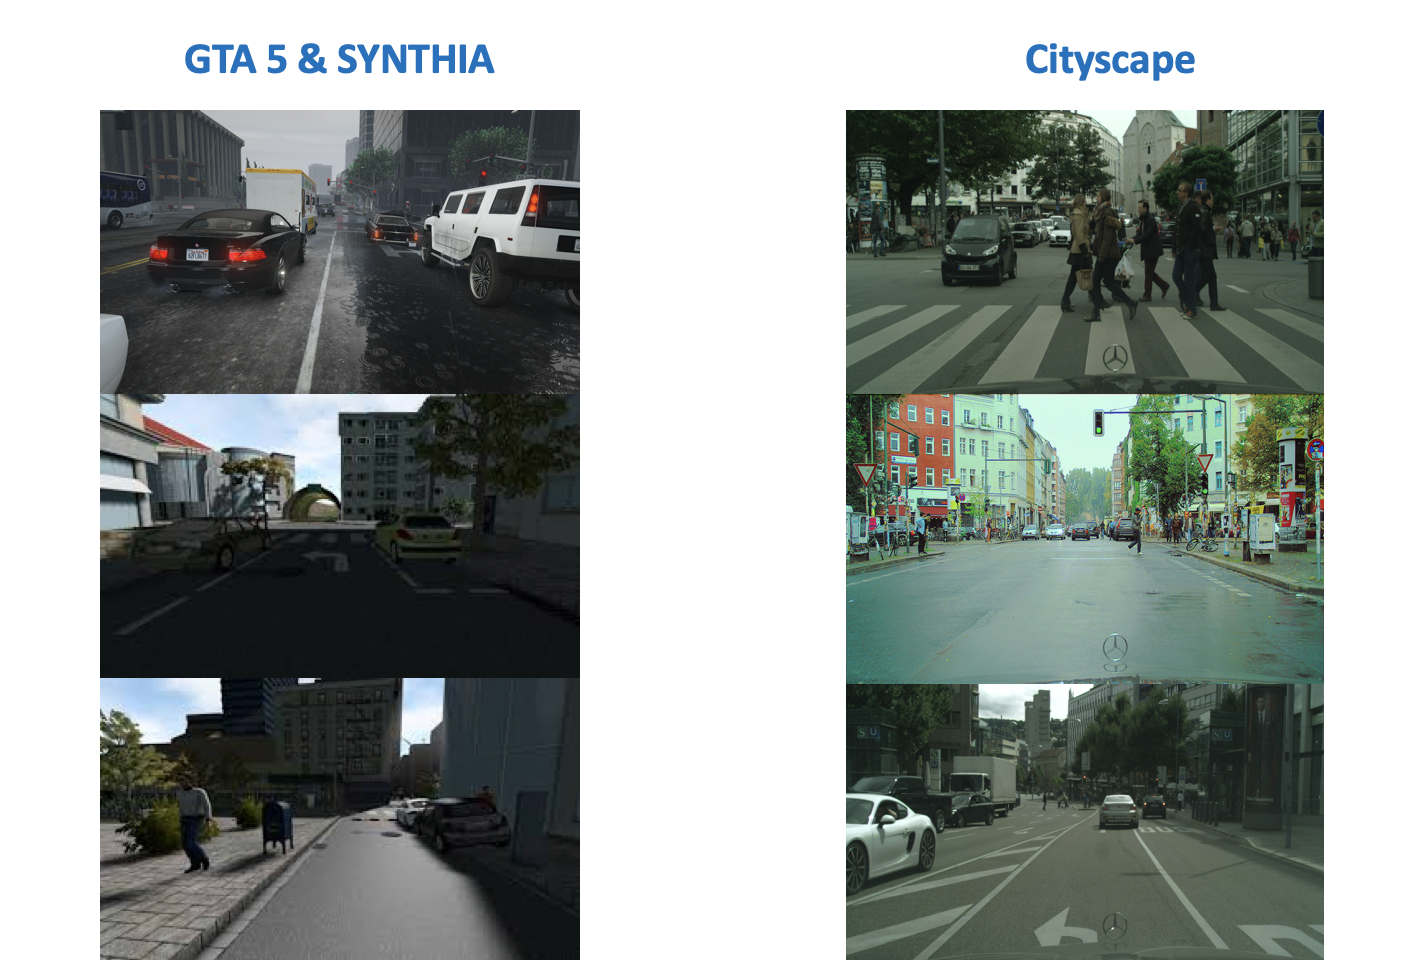
\includegraphics[scale=0.3]{images/domains_example.png}
    \caption{Два домена: синтетические и реальные виды города}
    \label{fig:domains-example}
\end{figure}

Сильным развитием данной задачи послужила, частная формулировка трансляции домена, а именно генеративное моделирование. Пусть дан наблюдаемый набор данных $Y$, элементы, $y$, которого принадлежат базовому распределению $y \sim \pi_y$. Цель любой генеративной модели состоит в том, чтобы аппроксимировать это распределение данных при наличии доступа к $Y$. После обучения, такая модель позволяет генерировать новые объекты $\hat y \notin Y$.

Так, например, состязательные сети (GAN), предложенные Гудфуллоу в статье \cite{gan}, стали основой одного из значимых методов в задаче трансляции домена. В GAN обучается две модели генератор и дискриминатор, первая из которых пытается сгенерировать реалистичные данные, а вторая пытается определить, является ли данные реальными или сгенерированными. Разработанный подход позволяет обучать неявным образом генеративные распределения, используя только сэмплы из реального распределения данных $p_y$. Методом, который обобщает GAN на задачу трансляции доменов, является CycleGAN, предложенный в \cite{cycle-gan}. Данный метод обучает два GAN, которые отображают данные в элементы противоположного набора.

Следующий класс генеративных моделей, адаптированных на задачу трансляции домена, стали диффузионные модели \cite{ddpm}. Они полагаются на итеративную процедуру, при которой распределение данных $p_{data}$ сначала искажается с помощью процесса прямого зашумления, сходящегося к нормальному распределению. Затем изучается обратный во времени процесс, который восстанавливает данные из гауссовского распределения обратно в распределение данных, с использованием score matching подходов. Для обобщения данной задачи важную роль сыграло понимание ограничений, а именно фиксированного нормального распределения, которое является не самым оптимальным выбором скрытого пространства. Например, для задачи восстановления зашумленных изображение, имея соответсвующее изображение высокого качества, имеет смысл восстанавливать начиная с зашумленного. Однако, это требует изменения целевого распределения прямого процесса, что часто неразрешимо и приводит к численным трудностям. 

В качестве обобщения диффузионных моделей на задачу трансляции домена был предложен метод Bridge matching \cite{bridge-matching}. Аналогично с диффузионными моделями данный метод, строит два стохастических процесса, прямой и обратный, между двумя маргинальными распределениями, таким образом обобщая задачу на два заданные произвольные распределения.

Однако вышеуказанны подходы обладают рядом недостатков. Во-первых, для Bridge matching требуются специализированные наборы данных, объекты которых являются пары из двух заданных конечных распределений, то есть во время обучения оба элемента пары должны соответствовать одному объекту, например, изображение представленное в двух видах: зашумленное и высокого качества. Во-вторых, в данных методах никак не задается оптимальность отображений. В статье \cite{translation-optimality} показывается, что данные методы ориентированы на небольшие преобразования. Это не является проблемой, когда распределения близки друг к другу, но в обратной ситуации, это не позволяет уловить более сложную семантику распределений. Таким образом, возникает потребность внедрять информацию о данных, что требует для каждой задачи адаптировать целевую функцию. 

Решением этих проблем является введение дополнительные критериев оптимальности отображений. Такими требованиями обладают мосты Шрёдингера \cite{schrödinger}, \cite{leonard-survey}. Задача мостов Шрёдингера находит стохастический процесс (рисунок \ref{fig:bridges_example}), ограниченный двумя заданными конечными распределениями, который наиболее похож с винеревским процессом с точки зрения дивергенции Кульбака — Лейблера. Такая формулировка задачи позволяет находить отображения между двумя непарными наборами данных, а также наиболее оптимальным образом, с точки зрения квадрата расстояния между элементами. Кроме того, данная задача позволяет вычислять вероятность этого стохастического процесса, что позволяет нам сравнивать два набора данных, что может быть полезно для проверки гипотез и семантического сходства.

\begin{figure}
    \centering
    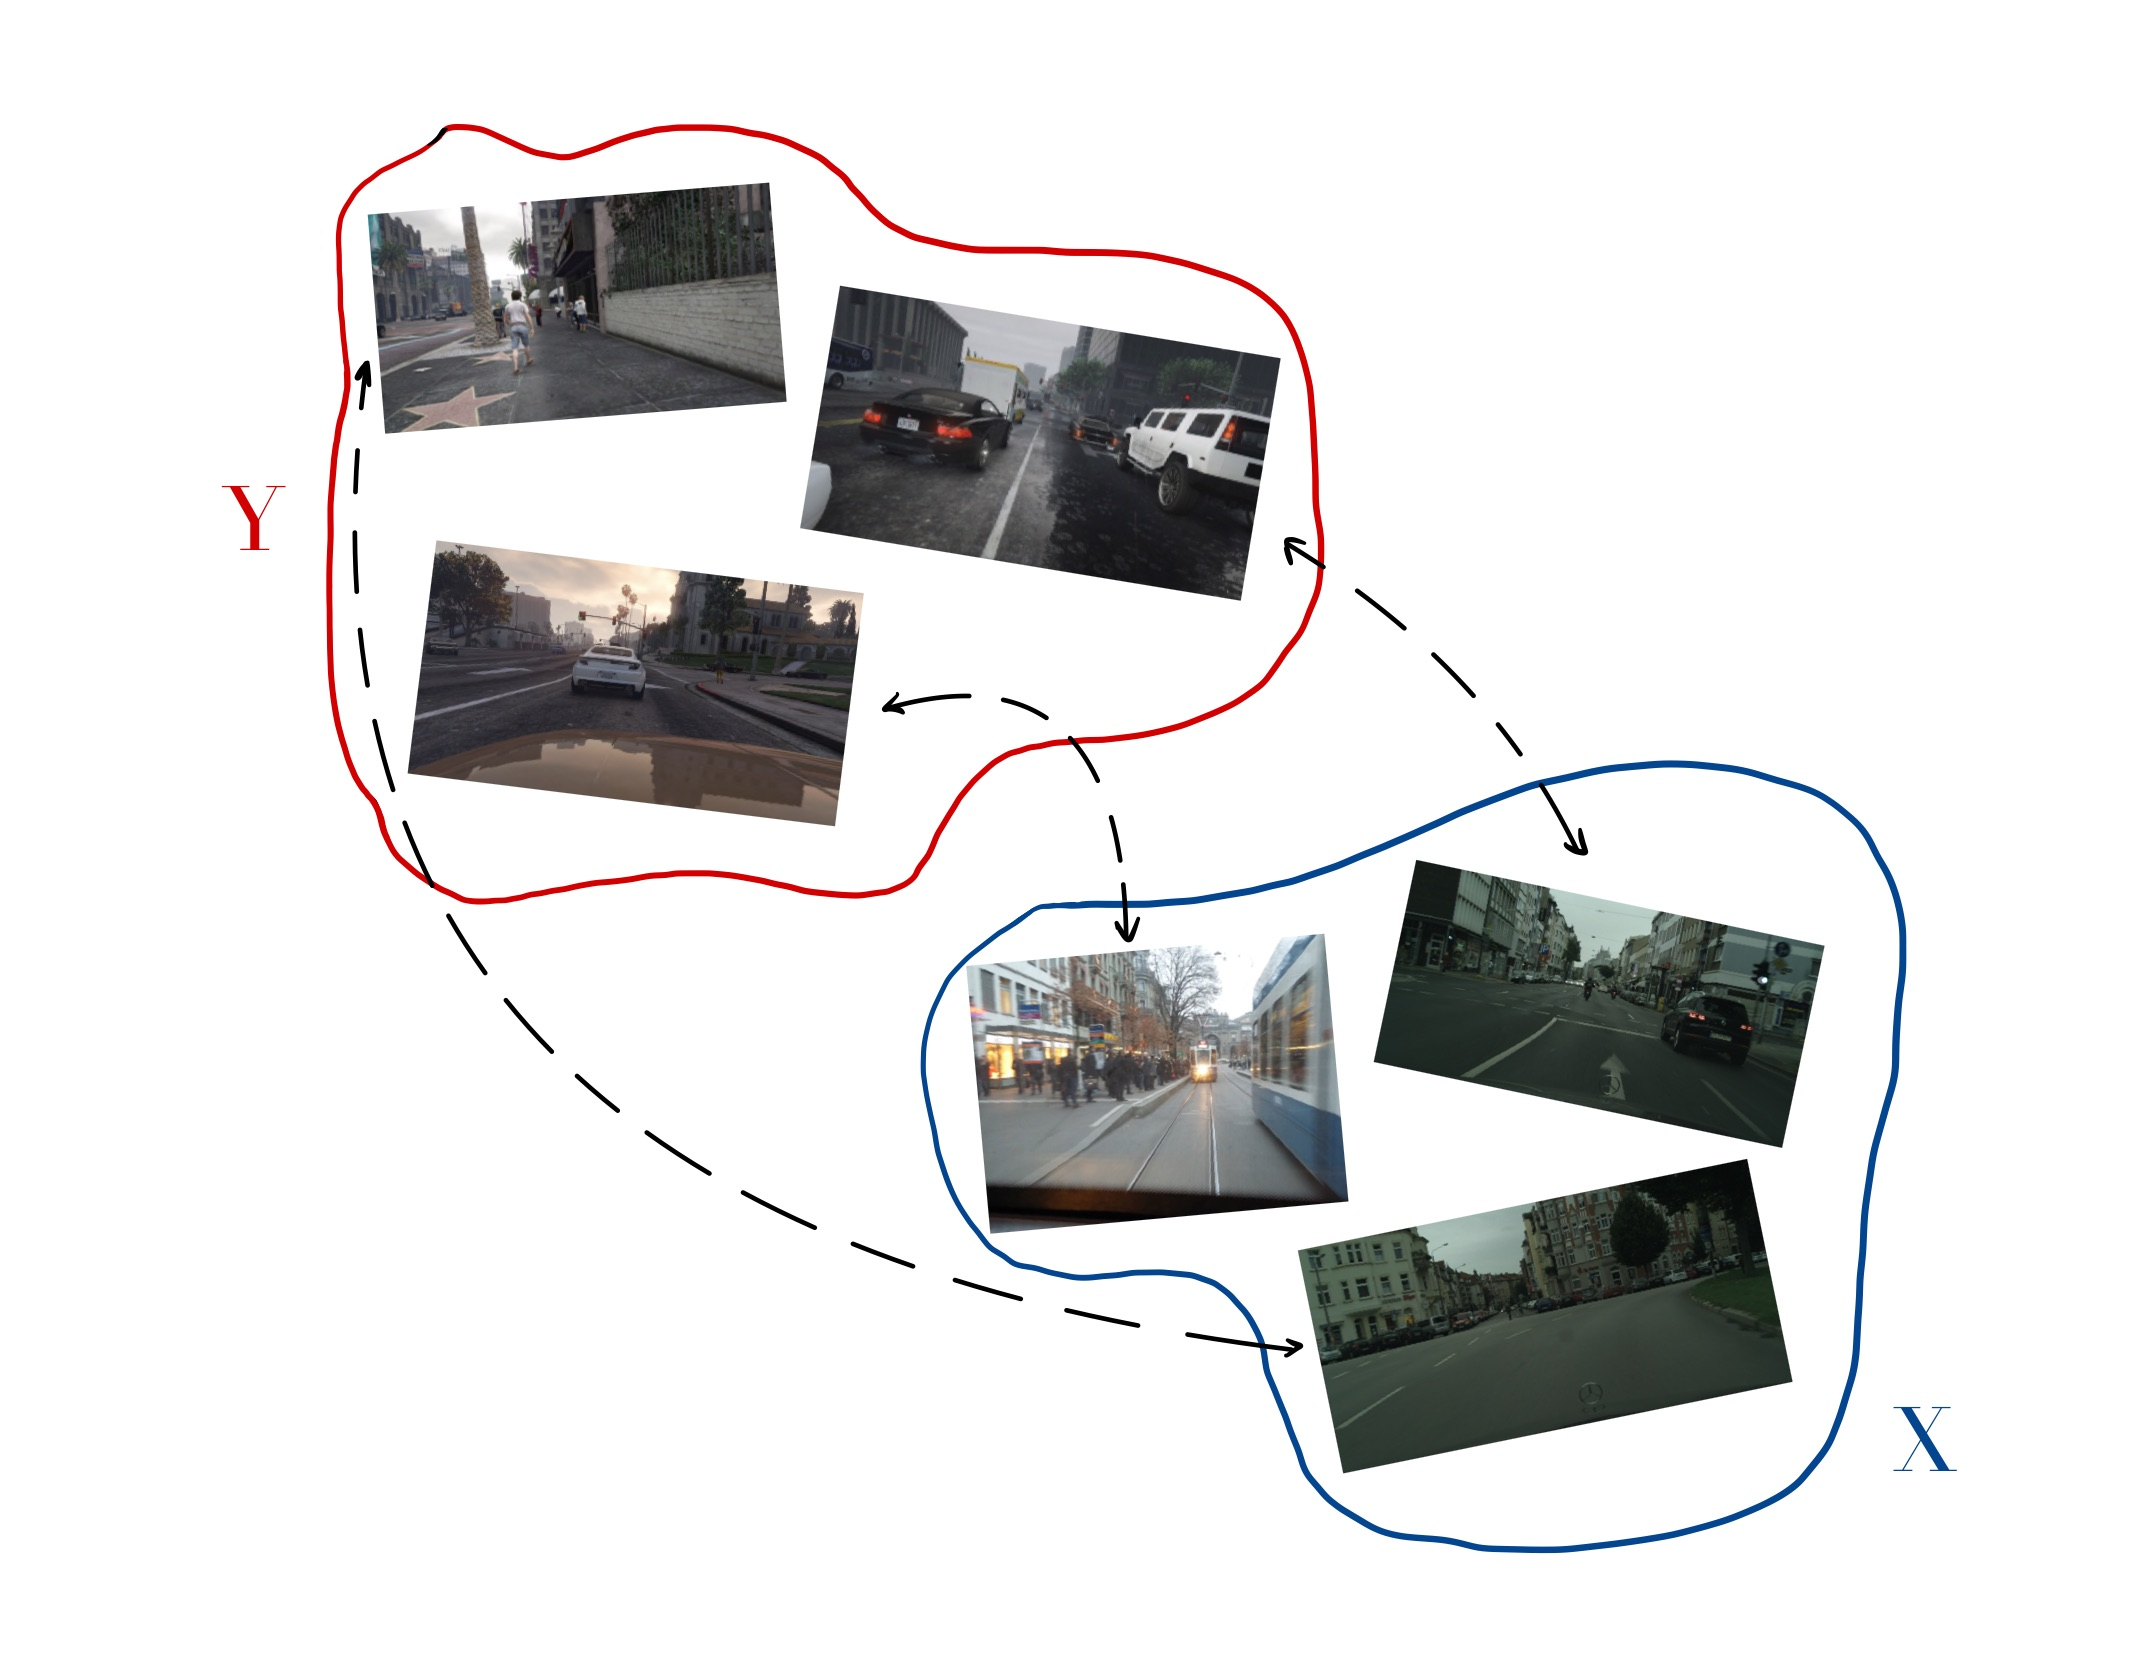
\includegraphics[scale=0.2]{images/bridges_example.jpg}
    \caption{Иллюстрация мостов Шрёдингера}
    \label{fig:bridges_example}
\end{figure}

Также, несомненная актуальность исследований в сфере мостов Шрёдингера подтверждается количеством статей, публикуемых в данное время. Так по запросу сайта arXiv\footnote{https://arxiv.org/} количество статей за последние 12 месяцев составило 56, когда год назад за такой же промежуток времени результат оказался в два раза меньше и составил 23 статьи.

Из-за родства диффузионных генеративных моделей с мостами Шрёдингера было предложено несколько подходов \cite{dsb}, \cite{dsbm}, \cite{mle-sb}, \cite{cycle-sb}. Несмотря на качество полученных результатов подходы предложенные в этих статьях являются вычислительно-дорогостоящими из-за этого возникает потребность в использовании других методов построения мостов Шредингера. 

Одними из примеров работ, которые не обладают данной проблемой, являются подходы описанные в следующих статьях \cite{lsb} и \cite{pavon-empiric-fortret}. Однако данные методы обладают другой проблемой: они страдают от проклятия размерности. Первый, несмотря на значительную скорость обучения, не предназначен для работы с такими данными. А второй метод, из-за особенностей оценивания интеграла, становится сложно вычислимым для данных большой размерности.

Благодаря исследованиям состязательных генеративных сетей \cite{fgan}, а именно доказательству, что целевая функция GAN может быть обобщена до f-семейства дивергенций, в данной работе предлагается новый подход к обучению мостов Шредингера, который наследует преимущества состязательных генеративных сетей и решает вышеперечисленные проблемы.

\newpage
 %% Введение
    \section{Задача Мостов Шредингера}
\label{sec:Chapter1} \index{Chapter1}
Существует несколько эквивалентных задач мостов Шрёдингера. Для понимания проблематики актуальных решений и перед тем как перейти к постановки задачи и предложенному методу решения, потребуется рассмотреть их, а также итеративные алгоритмы решения данных задач. Для этого, сначала потребуется ввести определение меры пути.

\begin{definition}[Мера пути]
    Для процесса Ито вида 
    \begin{equation*}
        dx(t) = b(t) + \sigma(t)d\beta(t),
    \end{equation*}

    определенного на интервале $[0, T]$, с функция сноса -- $b(t)$, $\sigma(t)$ -- функция волатильности, $\mathbb{P}$ называется мерой пути данного процесса с пространством исходов $\Omega = C([0, T], \mathbb{R}^d)$, если распределение $\mathbb{P}$ описывает слабое решение данного стохастического дифференциального уравнения (СДУ).
\end{definition}

Иначе говоря, мера пути представляет собой меру вероятности, ассоциированную со случайным процессом, задаваемым СДУ. Например, $\mathbb{W}^\gamma$ является мерой Винера и представляет вероятность траекторий винеровского процесса с волатильностью $\sqrt{\gamma}$ то есть $dx(t) = \sqrt{\gamma}d\beta(t)$.

\subsection{Динамическая постановка задачи мостов Шрёдингера}
Задача мостов Шрёдингера возникает из вопроса: как ограничить некоторый заданный случайный процесс? Ответ дает теория больших отклонений, в частности, теорема Санова \cite{sanov}.

\begin{theorem}[Санов]
    Пусть заданы $\{x_i(t)\}^N_{i=1}\sim \mathbb{W}^\gamma$ -- независимые одинаково распределённые траектории из меры пути априорного винеревского процесса $\mathbb{W}^\gamma$, где $x_i (t) \in \mathcal{C}([0,T], \mathbb{R}^d), \forall i=\overline{1, N}$. Также пусть дана эмпирическая мера $\hat{\mathbb{W}}$ по заданным траекториям:
    \begin{equation*}
        \hat{\mathbb{W}}(A)=\frac{1}{N}\sum_{i=1}^N\mathds{1}\left(x_i(t)\in A\right), A\in \mathcal{B}(\mathbb{R}^d)^{[0,T]},
    \end{equation*}
    тогда вероятность, что $\hat{\mathbb{W}}$ ограничена заданными распределениями $\pi_0$ и $\pi_T$ задана следующей асимптотической оценкой:
    \begin{equation}
        P\left(\hat{\mathbb{W}} \in \mathcal{D}(\pi_0, \pi_T)\right) \xrightarrow{N\rightarrow \infty} \exp\left(-N\inf_{\mathbb{Q} \in \mathcal{D}(\pi_0, \pi_T)}D_{KL}\mathbb{(Q||W})\right),
        \label{eq:sanov-theorem}
    \end{equation}
    где $\mathcal{D}(\pi_0, \pi_T)$ -- множество всех мер путей ограниченных заданными распределениями $\pi_0$ и $\pi_T$.
\end{theorem}

Таким образом, для того, чтобы ограничить $\hat{\mathbb{W}}$ распределениями $\pi_0$ и $\pi_T$, необходимо:
\begin{equation*}
    P\left(\hat{\mathbb{W}} \in \mathcal{D}(\pi_0, \pi_T)\right) = 1,
\end{equation*}
следовательно, степень экспоненты должна быть нулевой. Для этого необходимо, чтобы дивергенция меры пути совпадали и Кульбака-Лейблера была нулевой.

Первой постановкой является динамическая. Она прямо следует из асимптотической оценки Санова \ref{eq:sanov-theorem} и находит такую меру пути $\mathbb{Q}$, ограниченную заданными распределениями $\pi_0(x)$ и $\pi_T(y)$, что наиболее близка с точки зрения теории информации к априорной мере пути винеровского процесса $\mathbb{W}^\gamma$ с волатильностью $\sqrt\gamma$:
\begin{equation}
    \hat{\mathbb{Q}} = \arg\min_{\mathbb{Q}\in \mathcal{D}(\pi_0, \pi_T)} D_{KL}\mathbb{(Q||W}^\gamma)
    \label{dyn}
\end{equation}

\subsection{Статическая постановка мостов Шрёдингера}
Помимо динамической постановки также существует и статическая. Для её вывода и доказательства эквивалентности рассмотрим декомпозицию дивергенции Кульбака-Лейблера в уравнении \ref{dyn}. Сначала выразим производную Радона-Никодима, условную по $\textbf{x}(0)=x$ и $\textbf{x}(T)=y$:
\begin{equation*}
    \frac{d\mathbb{Q}}{d\mathbb{W}^\gamma} = \frac{q(x, y)}{p^{\mathbb{W}^\gamma}(x, y)}\frac{d\mathbb{Q}_{(0,T)}}{d\mathbb{W}^\gamma_{(0,T)}}(\cdot|x,y)
\end{equation*}

Подставляя это выражение в дивергенцию Кульбака-Лейблера в уравнении \ref{dyn}, получаем:
\begin{equation*}
    \begin{split}
        D_{KL}\mathbb{(Q||W}^\gamma) = \mathbb{E_Q}\left[\log \frac{d\mathbb{Q}}{d\mathbb{W}^\gamma}\right] = \mathbb{E_Q}\left[\log \frac{q(x, y)}{p^{\mathbb{W}^\gamma}(x, y)}\frac{d\mathbb{Q}_{(0,T)}}{d\mathbb{W}^\gamma_{(0,T)}}(\cdot|x,y)\right] = \\ = \int\log \frac{q(x, y)}{p^{\mathbb{W}^\gamma}(x, y)} d\mathbb{Q} + \int\log \frac{d\mathbb{Q}_{(0,T)}}{d\mathbb{W}^\gamma_{(0,T)}}(\cdot|x,y)d\mathbb{Q}= \\ = \int q(x, y)\log \frac{q(x, y)}{p^{\mathbb{W}^\gamma}(x, y)} dxdy + \int\log q(x, y)\frac{d\mathbb{Q}_{(0,T)}}{d\mathbb{W}^\gamma_{(0,T)}}(\cdot|x,y)d\mathbb{Q}_{(0,T)} = \\ = D_{KL}\left(q(x, y) || p^{\mathbb{W}^\gamma}(x, y)\right) + \mathbb{E}_{q(x, y)}\left[D_{KL}\left(\mathbb{Q}_{(0,T)}(\cdot|x,y) || \mathbb{W}^\gamma_{(0,T)}(\cdot|x,y)\right)\right]
    \end{split}
\end{equation*}

Видно, что второй член дивергенции Кульбака-Лейблера не учитывает маргинальные распределения, поэтому он не влияет на оптимизационные ограничения и может быть отброшен. Таким образом, не рассматривается динамика на интервале $(0, 1)$ и для решения задачи важно только совместное распределение между крайними маргинальными распределениями. 

В результате получается статическая постановка задачи мостов Шрёдингера:
\begin{equation}
    \left\{ 
    \begin{array}{c}
        \hat q(x,y) = \arg\min_{q(x,y)} D_{KL}(q(x,y)||p^{\mathbb{W}^\gamma}(x,y)), \\
        \pi_0(x) = \int q(x,y)dy, \\
        \pi_T(y) = \int q(x,y)dx,
        \label{static}
    \end{array}\right.
\end{equation}
где $q(x,y)$ — это совместное распределение, которое является ближайшим к броуновскому движению при условии ограничений на маргинальные распределения. 

\subsection{Система Шрёдингера}
Третья формулировка требует рассмотрения лагранжиана статической постановки \ref{static}:
\begin{equation*}
    \begin{split}
        L(q, \lambda, \mu) = D_{KL}(q(x,y)||p^{\mathbb{W}^\gamma}(x,y)) + \int \lambda(x)\left(\int q(x, y)dy - \pi_0(x)\right)dx + \\ + \int \mu(y)\left(\int q(x, y)dy - \pi_T(y)\right)dy
    \end{split}
\end{equation*}

Предполагая, что $p^{\mathbb{W}^\gamma}(x,y) = p_0^{\mathbb{W}^\gamma}(x)p^{\mathbb{W}^\gamma}(y|x)$, где $p_0^{\mathbb{W}^\gamma}(x)$ может быть любым, а так как априорный процесс является винеровским, $p^{\mathbb{W}^\gamma}(y|x)=\mathcal{N}(y|x, \gamma I_d)$, приравняем $\frac{\partial L(q, \lambda, \mu)}{\partial q(x,y)}$ нулю и получим:
\begin{equation*}
    q^*(x, y) = \exp{(\ln{p^{\mathbb{W}^\gamma}(x,y)} - \lambda(x) - 1)}p^{\mathbb{W}^\gamma}(y|x)\exp{(-\mu(y))}
\end{equation*}

Теперь положив, что  $\hat\phi_0(x) = \exp{(\ln{p^{\mathbb{W}^\gamma}(x,y)} - \lambda(x) - 1)}$ и $\phi_T(y) = \exp{(-\mu(y))}$ получаем:
\begin{equation*}
    q^*(x, y) = \hat\phi_0(x)p^{\mathbb{W}^\gamma}(y|x)\phi_T(y),
\end{equation*}
удовлетворяющее:
\begin{equation*}
    \hat{\phi}_0(x) \int \phi_T(y) p_W^\gamma(y|x) dy = \pi_0(x),
\end{equation*}
\begin{equation*}
    \phi_T(y) \int \hat{\phi}_0(x) p_W^\gamma(y|x) dx = \pi_T(y),
\end{equation*}

Теперь переобозначим термины с интегралами как:
\begin{equation*}
    \phi_0(x) = \int \phi_T(y) p_W^\gamma(y|x) dy,
\end{equation*}
\begin{equation*}
    \hat{\phi}_T(y) = \int \hat{\phi}_0(x) p_W^\gamma(y|x) dx.
\end{equation*}

Объединяя все вместе, следующая линейная функциональная система является системой Шрёдингера:
\begin{equation}
    \left\{ 
    \begin{array}{c}
        \hat{\phi}_0(x) \phi_T(x) = \pi_0(x), \\
        \hat{\phi}_T(x) \phi_T(y) = \pi_T(y).
    \label{sys_sb}
    \end{array}\right.
\end{equation}

\subsection{Динамические полумосты Шрёдингера}
Наиболее важной для этой работы является постановка задачи полумостов Шрёдингера. В отличии от оригинальной задачи мостов Шрёдингера, задача полумостов ограничивается только на одну сторону, то есть $\mathcal{D}(\pi_0(x), \cdot)$ или $\mathcal{D}(\cdot, \pi_T(y))$. 

Более формально задача прямого полумоста, то есть, ограниченного в момент времени 0, определяется так:
\begin{equation}
    \mathbb{Q}^*=\arg\min_{\mathbb{Q}\in\mathcal{D}(\pi_0(x), \cdot)}D_{KL}\left(\mathbb{Q}||\mathbb{W}^\gamma\right),
    \label{eq:forward_hsb}
\end{equation}
а задача обратного определятся следующим образом:
\begin{equation}
    \mathbb{P}^*=\arg\min_{\mathbb{P}\in\mathcal{D}(\cdot, \pi_T(y))}D_{KL}\left(\mathbb{P}||\mathbb{W}^\gamma\right)
    \label{eq:backward_hsb}
\end{equation}

В отличии от оригинальной постановки задачи мостов Шрёдингера, задачи обоих полумостов имеет следующее аналитическое решение:
\begin{equation*}
    \mathbb{Q}^*(A_0\times A_{(0,1]})=\int_{A_0\times A_{(0,1]}}\frac{d\pi_0}{p_0^{\mathbb{W}^\gamma}}(x)d\mathbb{W}^\gamma
\end{equation*}
\begin{equation*}
    \mathbb{P}^*(A_{[0,T)} \times A_T)=\int_{A_{[0,T)} \times A_T}\frac{d\pi_T}{p_T^{\mathbb{W}^\gamma}}(y)d\mathbb{W}^\gamma,
\end{equation*}
для прямого и обратного мостов соответственно.

\subsubsection{Статические полумосты Шрёдингера}
Аналогично и оригинальной постановке рассмотрим статическую формулировку полумостов. Прямой полумост задается следующим образом:
\begin{equation}
    \begin{split}
        q^*(x,y)=\arg\min_{q(x,y)\in\mathcal{D}(\pi_0(x), \cdot)}D_{KL}\left(q(x,y)||p^{\mathbb{W}^\gamma}(x,y)\right), \\
        \text{такое, что } \pi_0(x) = \int q(x, y)dy,
    \end{split}
\end{equation}
а обратный:
\begin{equation}
\begin{split}
    p^*(x,y)=\arg\min_{p(x,y)\in\mathcal{D}(\cdot, \pi_T(y))}D_{KL}\left(p(x,y)||p^{\mathbb{W}^\gamma}(x,y)\right), \\
    \text{такое, что } \pi_T(y) = \int q(x, y)dx.
\end{split}
\end{equation}

Как и для динамической постановки статическая обладает аналитическим решением:
\begin{equation*}
    q(x,y)^*=p(x,y)^{\mathbb{W}^\gamma}\frac{\pi_0(x)}{p^{\mathbb{W}^\gamma}(x)},
\end{equation*}
\begin{equation*}
    p(x,y)^*=p(x,y)^{\mathbb{W}^\gamma}\frac{\pi_T(y)}{p^{\mathbb{W}^\gamma}(y)},
\end{equation*}
для прямого и обратного полумостов, соответственно.

Полумосты полезны не только из-за того, что обладают аналитическим решением, но и тем, что позволяют легко справится с ограничением на искомый мост, заменяя его на задачу с начальным значением. Также благодаря полумостам итеративною решается оригинальная задача мостов Шрёдингера.

\subsection{Методы решения мостов Шрёдингера}
Далее рассмотрим итеративные алгоритмы, которые решаяют задачу мостов Шрёдингера.

Алгоритм Фортета \ref{alg:fortret} является одним из старейших методов, доказавших свою сходимость для решения системы Шрёдингера. Этот алгоритм, впервые предложенный Фортетом в 1940 году \cite{fortret}, включает итеративный процесс, обеспечивающий выполнение маргинальных условий системы Шрёдингера \ref{sys_sb} для распределений в моменты времени $t=0$ и $t=T$.

\begin{algorithm}
\caption{Фортет}\label{alg:fortret}
\KwInput{$\pi_0(x)$, $\pi_T(y)$, $p(y|x)$}
\KwOutput{$\hat\phi^{(i)}_0(x)$, $\phi^{(i)}_T(y)$}
Инициализируем $\phi_0^{(0)}(x)$ такое, что $\phi_0^{(0)}(x)<<\pi_0(x)$\;
Инициализируем $i = 0$\;
\While{не сойдется}{
    $\hat\phi_0^{(i)}(x):=\frac{\pi_0(x)}{\phi_0^{(i)}(x)}$\;
   $\hat\phi_T^{(i)}(y):=\int p(y|x)\hat\phi_0^{(i)}(x)dx$\;
    $\phi_T^{(i)}(y):=\frac{\pi_T(y)}{\hat\phi_T^{(i)}(y)}$\;
    $\hat\phi_T^{(i+1)}(x):=\int p(y|x)\phi_T^{(i)}(y)dy$\;
    $i:=i+1$\;
   }
\end{algorithm}

Алгоритм Фортета фактически чередует выполнение маргинальных условий для моментов времени $t=0$ и $t=T$, пока не сойдется. В результате достигается решение, соответствующее заданным граничным условиям для обоих моментов времени.

Другим методом решения задачи мостов Шрёдингера является алгоритм Iterative Proportional Fitting (IPF). IPF -- это метод, используемый для нахождения дискретное совместное распределение при заданных маргинальных, используя принципы максимальной энтропии. Однако в контексте мостов Шрёдингера, а именно статической постановки задачи, в 1968 году Кульбаком \cite{kullback} был разработан непрерывный вариант IPF, а сходимость его доказана Рушендорфом \cite{kullback-prove}.

\begin{algorithm}
\caption{IPF}\label{alg:ipfp}
\KwInput{$\pi_0(x)$, $\pi_T(y)$, $p(y|x)$}
\KwOutput{$q_i^*(x, y), p_i^*(x, y)$}
Инициализируем $p_T^{\mathbb{W^\gamma}}(y)$ такое, что $p_T^{\mathbb{W^\gamma}}(y)<<\pi_T(y)$\;
Инициализируем $q_0^*(x,y) := p^{\mathbb{W}^\gamma}(x,y)$\;
Инициализируем $i = 0$\;
\While{не сойдется}{
    $p_i^*(x,y) = \arg\min_{p(x,y)\in \mathcal{D}(\cdot, \pi_T(y))}D_{KL}(p(x,y)||q^*_{i-1}(x,y))$\;
    $q_i^*(x,y) = \arg\min_{q(x,y)\in \mathcal{D}(\pi_0(x), \cdot)}D_{KL}(q(x,y)||p^*_i(x,y))$\;
    $i:=i+1$\;
   }
\end{algorithm}

\begin{figure}
    \centering
    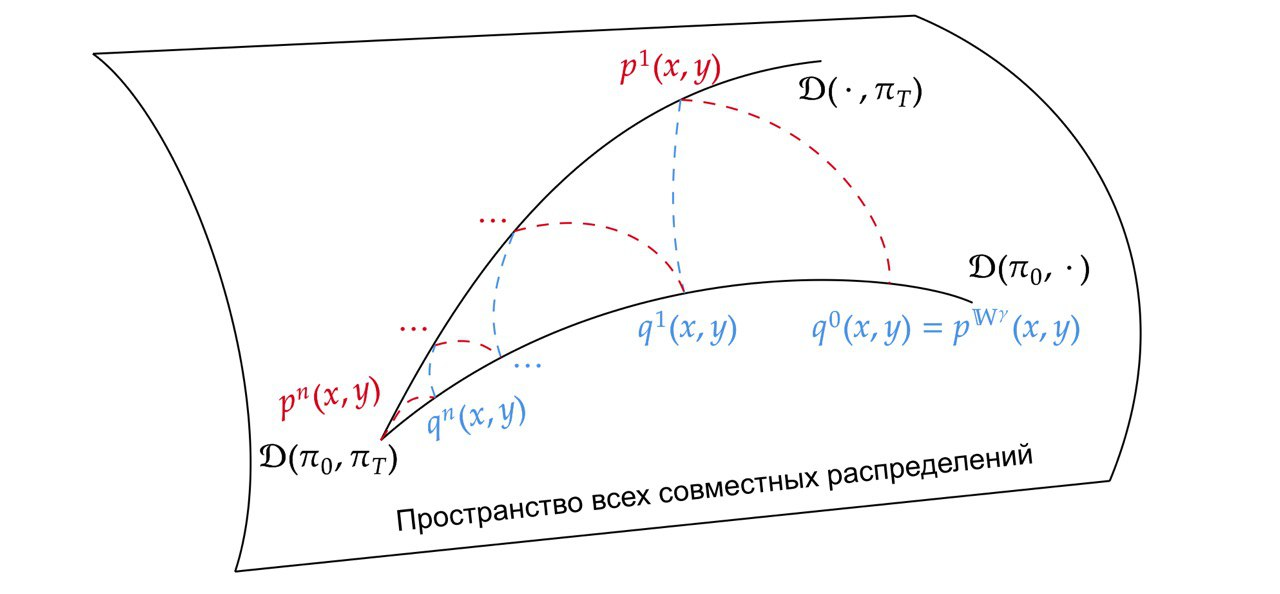
\includegraphics[width=1\linewidth]{images/ipfp.png}
    \caption{Иллюстрация алгоритма IPF}
    \label{fig:ipfp}
\end{figure}

Суть алгоритма Кульбака заключается в чередовании решения полумостов начиная с обратного. Можно заметить, что если шаги 5 и 6 переписать с помощью аналитического решения задачи полумостов, а также начать алгоритм с прямого прохода, данный алгоритм сводится к алгоритму Фортета. Иллюстрация IPFP изображена на рисунке \ref{fig:ipfp}

Следующий алгоритм generalised IPF (g-IPF) обобщает IPF, предложенный Кульбаком, применяя его к динамической постановке задачи. Этот метод идентичен обычному IPF, однако на каждом шаге минимизируется дивергенция Кульбака-Лейблера между двумя мерами путей. 
\newpage
\begin{algorithm}
\caption{g-IPF}\label{alg:g-ipfp}
\KwInput{$\pi_0(x)$, $\pi_T(y)$, $\mathbb{W}^\gamma$}
\KwOutput{$\mathbb{Q}_i^*(x, y), \mathbb{P}_i^*(x, y)$}
Инициализируем $\mathbb{Q}_0^*(x,y) := \mathbb{W}^\gamma$\;
Инициализируем $i = 0$\;

\While{не сойдется}{
    $\mathbb{P}_i^*(x,y) = \arg\min_{\mathbb{P}(x,y)\in \mathcal{D}(\cdot, \pi_T(y))}D_{KL}(\mathbb{P}(x,y)||\mathbb{Q}^*_{i-1}(x,y))$\;
    $\mathbb{Q}_i^*(x,y) = \arg\min_{\mathbb{Q}(x,y)\in \mathcal{D}(\pi_0(x), \cdot)}D_{KL}(\mathbb{Q}(x,y)||\mathbb{P}^*_i(x,y))$\;
    $i:=i+1$\;
   }
\end{algorithm}

\newpage %% Постановка задачи
    \section{Постановка задачи}
\label{sec:Chapter2} \index{Chapter2}

В контексте машинного обучения зачастую невозможно получить распределение данных в явной форме. Это вызывает необходимость рассмотрения альтернативных постановок задачи мостов Шрёдингера, в которых маргинальные распределения известны лишь посредством выборок, представленных в виде двух наборов данных $\{x_i\}_{i=0}^N = X \in \mathbb{R}^{N\times d}$ и $ \{y_j\}_{j=0}^M = Y\in \mathbb{R}^{M\times d}$. 

Эмпирическими мостами Шрёдингера называется такая постановка задачи мостов Шрёдингера, в которой маргинальные распределения известны только через выборки (то есть их эмпирические распределения):

\begin{equation*}
    \hat{\pi}_0(x) = \frac{1}{N} \sum_{i=1}^{N} \delta(x - x_i), \quad \hat{\pi}_T(y) = \frac{1}{M} \sum_{j=1}^{M} \delta(y - y_j),
\end{equation*}
где $\delta$ -- дельта-функция Дирака.

Элементы этих наборов принадлежат соответствующим распределениям, а именно $x_0 = x \sim \pi_0(x)$ и $x_T = y \sim \pi_T(y)$.
Проанализировав существующие подходы, можно заключить, что большинство методов, таких как Diffusion Schrödinger Bridge \cite{dsb}, Iterative Proportional Maximum Likelihood (IPML) \cite{mle-sb} и Unpaired Neural Schrödinger Bridge \cite{cycle-sb}, основываются на моделировании дискретизированного стохастического процесса, представленного марковской цепочкой:
\begin{equation*}
q(x_0, \dots, x_T) = \pi_1(x_T) \prod_{t=0}^{T-1} q_{t|t+1} (x_t | x_{t+1}).
\end{equation*}

В этих методах условное распределение $q_{t|t+1}$ параметризуется с использованием нейронных сетей. Для преобразования одного набора данных в другой в этих методах итеративно сэмплируются элементы с использованием обученного $q_{t|t+1}$, таким образом моделируя стохастический процесс. В результате таких преобразований требуется несколько шагов для переноса элемента из одного набора в другой. Несмотря на значительный прогресс в сокращении числа необходимых шагов, такие методы все еще являются вычислительно сложными задачами.

С другой стороны, методы, которые рассматривают задачу мостов Шрёдингера без моделирования процесса, такие как Data Driven Schrödinger Bridge \cite{pmlr-v139-wang21l} и Light Schrödinger Bridge \cite{lsb}, плохо справляются с данными большой размерности из-за необходимости явной параметризации и обучения условного распределения.

В связи с этим, возникает необходимость разработки подхода к решению задачи мостов Шрёдингера, который бы обладал следующими качествами:
\begin{itemize}
\item преобразование из одного распределения в другое должно осуществляться за один шаг;
\item метод должен быть эффективным при работе с данными большой размерности.
\end{itemize}

Таким образом, цель данной работы состоит в предложении решения задачи мостов Шрёдингера, которое бы удовлетворяло указанным выше требованиям. 

\newpage %% Обзор существующих решений
    \section{Обзор существующих решений задачи мостов Шрёдингера}
\label{sec:Chapter3} \index{Chapter3}

Для более полного анализа поставленной проблемы, далее рассматриваются существующие методы решения задачи эмпирических мостов Шрёдингера.

\subsection{Data Driven Schrödinger Bridge}
Подход, предложенный в статье \cite{pavon-empiric-fortret}, является адаптацией алгоритма \ref{alg:fortret} к эмпирической постановке. Данный метод основан на том факте факте, что шаги 4 и 6 \ref{alg:fortret}:
\begin{equation*}
    \begin{split}
    \hat{\phi}^{(i)}_0(x) := \frac{\pi_0(x)}{\phi^{(i)}_0(x)}, \\
    \phi^{(i)}_T(y) := \frac{\pi_T(y)}{\hat{\phi}^{(i)}_T(y)}
    \end{split}
\end{equation*}
могут быть эквивалентно сформулированы как проблема минимизации кросс-энтропии в пространстве распределений $\mathcal{H}$:
\begin{equation*}
    \begin{split}
        \hat{\phi}^{(i)}_0(x) = \arg \sup_{\phi_0(x) \in \mathcal{H}} \mathbb{E}_{\pi_0(x)} \left[ \ln \hat{\phi}_0(x) \phi^{(i)}_0(x) \right],\\
        \phi^{(i)}_T(y) = \arg \sup_{\phi_T(y) \in \mathcal{H}} \mathbb{E}{\pi_T(y)} \left[ \ln \phi_T(y) \hat{\phi}^{(i)}_T(y) \right].
    \end{split}
\end{equation*}

Далее, внедряя шаги 5 и 7 алгоритма \ref{alg:fortret} с помощью лагранжиана и параметризуя потенциалы с помощью смеси гауссиан, получают следующие два шага нового алгоритма:
\begin{equation*}
    \beta^{*}_i = \arg \max{\hat{\beta}} \frac{1}{M} \sum_{s} \ln \hat{\phi}_0(x_s; \hat{\beta}) \phi^{(i)}_0(x_s) - \int \hat{\phi}_0(x; \hat{\beta}) \phi^{(i)}_0(x) dx, \quad x_s \sim \pi_0(x),
\end{equation*}
и
\begin{equation*}
    \beta^{*}_i = \arg \max{\beta} \frac{1}{N} \sum_{s} \ln \phi_T(y_s; \beta) \hat{\phi}^{(i)}_T(y_s) - \int \phi_T(y; \beta) \hat{\phi}^{(i)}_T(y) dy, \quad y_s \sim \pi_T(y).
\end{equation*}

Далее декомпозируются ограничения введенные лагранжианом и оцениваются с помощью метода Монте Карло и выборки по значимости, и получают финальные оптимизационные задачи. Из-за проклятия размерности метода выборки по значимости, предложенный метод не масштабируется до данных с большой размерностью.

\subsection{Light Schrödinger Bridge}
Данный метод предложенный в \cite{lsb} решает задачу мостов Шрёдингера в статической формулировке \ref{static}, декомпозируя совместное распределение с помощью потенциалов:
\begin{equation*}
    \pi_{\theta}(x_0, x_1) = \pi_0(x) p^{\mathbb{W}^\gamma}(y|x) = \pi_0(x) \frac{p^{\mathbb{W}^\gamma}(y|x) \phi_T(y)}{\hat{\phi}_0(x)}.
\end{equation*}

Аналогично с предыдущим методом авторы параметризуют потенциалы с помощью смеси гауссиан. Далее авторы замечают, что данная декомпозиция позволяет сформулировать целевую функцию, минимизация которой эквивалентна минимизации дивергенции Кульбака-Лейблера:
\begin{equation*}
    L(\theta) = \int_{\mathbb{R}^D} \log \hat{\phi}_0(x) \pi_0(x)dx - \int_{\mathbb{R}^D} \log \phi_T(y) \pi_T(y) dy.
\end{equation*}

Напрямую решая задачу мостов Шрёдингера (без IPF), авторам удалось значительно ускорить обучения моделей, однако авторы комментируют, что такой метод не предназначен для работы с данными большой размерности.

\subsection{Diffusion Schrödinger Bridge}
Данный метод предложен Валентином Де Бортоли в статье \cite{dsb}. Автор рассматривает динамическую постановку задачи \ref{dyn} в дискретном виде, то есть вместо меры пути используют совместное распределение в точках стохастического процесса:
\begin{equation*}
    q^*(x_0, \ldots, x_T) = \arg \min_{q \in \mathcal{D}(\pi_0, \pi_T)} D_{KL}\left(q(x_0, \ldots, x_T) || p^{\mathbb{W}^\gamma}(x_0, \ldots, x_T)\right).
\end{equation*} 

Авторы доказывают, что формулировка задачи мостов Шрёдингера через совместные вероятности эквивалентна динамической постановке мостов Шрёдингера, у которой ассоциированный стохастический процесс дискретизирован с помощью метода Эйлера–Маруямы. Используя данный факт, авторы \cite{dsb} применяют алгоритм IPF, адаптированный к дискретной формулировке, для решения задачи мостов Шрёдингера. В результате основываясь на факте, что винеровский процесс является марковским, авторы формулируют минимизационные задачи IPF следующим образом:

\begin{equation}
    \begin{split}
        p^{i+1}(x_{0:T}) = \pi_0(x_0) \prod_{t=0}^{T-1} \left( \frac{q_{t|t+1}^i (x_t | x_{t+1}) q_{t+1}^i (x_{t+1})}{q_t^i (x_t)} \right),
        \\
        q^i(x_{0:T}) = \pi_T(x_T) \prod_{t=0}^{T-1} \left( \frac{p_{t+1|t}^i (x_{t+1} | x_t) p_t^i (x_t)}{p_{t+1}^i (x_{t+1})} \right).
    \end{split}
    \label{eq:dsb-prop2}
\end{equation}

Так как такую динамику смоделировать невозможно, условные вероятности $p_{t+1|t}^i(x_{t+1} | x_t)$ и $q_{t|t+1}^i (x_t | x_{t+1})$ представляют с помощью нормального распределения:
\begin{equation*}
    \begin{split}
        p_{t+1|t}^i (x_{t+1} | x_t) p_t^i (x_t) =  \mathcal{N}\left(x_{t+1};x_{t} + \gamma_{t+1}f^i_t(x_t), 2\gamma_{t+1}\mathbb{I}\right)
        \\
        q_{t|t+1}^i (x_t | x_{t+1}) = \mathcal{N}\left(x_{t};x_{t+1} + \gamma_{t}b^i_{t+1}(x_{t+1}), 2\gamma_{t}\mathbb{I}\right).
    \end{split}
\end{equation*}

Далее аппроксимировав с помощью ряда Тейлора, для \ref{eq:dsb-prop2} авторы получают:
\begin{equation*}
    \begin{split}
        p^{i+1}_{t+1|t}(x_{t+1} | x_t) \approx \mathcal{N}(x_{t+1}; x_t + \gamma_{t+1} f^{i+1}_t(x_t), 2 \gamma_{t+1} I), \\
        q^i_{t|t+1}(x_t | x_{t+1}) \approx \mathcal{N}(x_t; x_{t+1} + \gamma_{t+1} b^i_{t+1}(x_{t+1}), 2 \gamma_{t+1} I),        
    \end{split}
\end{equation*}
где
\begin{equation*}
    \begin{split}
        f^{i+1}_t(x_t) = -b^i_{t+1}(x_t) + 2 \nabla \log q^i_t(x_t), \\
        b^i_{t+1}(x_{t+1}) = -f^i_t(x_{t+1}) + 2 \nabla \log p^i_{t+1}(x_{t+1}).
    \end{split}
\end{equation*}

Затем логарифмы градиентов могут быть аппроксимированы с использованием score matching методов. Однако авторы, из соображений затрат памяти и вычислительной сложности аппроксимируют, среднее нормальных распределений \ref{eq:dsb-prop2}, то есть функции дрейфа ассоциированных стохастических процессов.

Благодаря применению задачи мостов Шрёдингера, авторам удалось сократить требуемое число диффузионных шагов в сравнении с score-based моделями. Так, например, для задач генерации изображений CelebA и MNIST для score-based моделей потребовалось 100 диффузионных шагов, а для предложенного метода \cite{dsb} 12.

\subsection{Iterative Proportional Maximum Likelihood (IPML)}
В работе \cite{mle-sb} авторы преобразуют алгоритм IPF в виде задачи максимума правдоподобия. Аналогично ранее описанной работе в данном методе используется тот факт, что мера пути в динамической постановке задачи мостов Шрёдингера, может быть параметризована с помощью функции сноса соответствующего стохастического дифференциального уравнения. Однако в место того, чтобы оценивать функцию сноса с помощью score matching подхода, авторы данного метода оценивают, используя гауссовские процессы.

Также, в отличии от метода \cite{pavon-empiric-fortret}, где оценка маргинальных распределений находится с помощью метода максимума правдоподобия, авторы данной работы находят оценку условного распределения, то есть смещения. В такой постановке не требуется оценивать интеграл с помощью метода Монте Карло, что позволяет работать с данными большой размерности. Однако не смотря на это, для отображения элементов из одного набора данных в другой, моделирует стохастический процесс.

\subsection{Unpaired Neural Schrödinger Bridge}
Наиболее близкий метод к предложенному в данной работе является подход описанный в статье \cite{cycle-sb}. Авторы рассматривают динамическую задачу мостов Шрёдингера и аналогично предыдущим методам параметризуют условное распределение $q(x_{t+1}|x_t)$. Однако, в отличии от них данный метод не использует IPF для обучения, что сильно упрощает оптимизационную задачу. 

Авторы выдоят следующую целевую функцию:
\begin{equation*}
    \begin{split}
        \min_{q} \mathcal{L}_{SB}(q, t) := \mathbb{E}_{q(x_{t_i}, x_T)} \left[ \|x_{t_i} - x_1\|^2 \right] - 2\tau(1 - t_i) H(q(x_{t_i}, x_T)) \\
        \text{такое, что} \quad \mathcal{L}_{Adv}(\phi_i; t_i) := D_{KL}(q(x_T) \| \pi_T(x_T)) = 0,
    \end{split}
\end{equation*}
где дополнительное условие рассматривается как регуляризация и минимизируется с помощью состязательного обучения. Далее доказывают, что оптимизация такой целевой функции находит решения задачи моста Шрёдингера.

Таким образом, несмотря на введение состязательного обучения, данный метод не решает проблему моделирования стохастического процесса.

\newpage
 %% Исследование и построение решения задачи
    \section{Исследование и построение решения задачи}
\label{sec:Chapter4} \index{Chapter4}

Исходя из требований, поставленных ранее, данным условиям соответствуют состязательные генеративные модели. Во-первых, они хорошо работают с данными большой размерности, достигая передовые результаты в задачах генерации изображений \cite{style-gan}, а во-вторых, генерация данных заключается в отображении элементов скрытого пространства в пространства данных, вызовом генератора, то есть за один шаг.

Для того чтобы связать состязательные генеративные модели с задачей мостов Шрёдингера, необходимо подробнее рассмотреть свойства и особенности GAN.

\subsection{Состязательные генеративные модели (Generative-adversarial networks, GAN) и их обобщение f-GAN}
В статье Гудфеллоу \cite{gan} был представлен новый метод оценки генеративных моделей с использованием состязательного обучения.

Такой метод обучает генеративную модель $G$ состязательно , вводя дискриминативную модель $D$, которая пытается определить, является ли выборка реальной или сгенерированной:
\begin{multline*}
    \min_{G}\max_{D}V(G, D) = \min_{G}\max_{D} \mathbb{E}_{x\sim p_{data}} [\log D(x)] - \mathbb{E}_{x\sim p_g} [1 - \log D(x)] = \\ = \min_{G}\max_{D} \mathbb{E}_{x\sim p_{data}} [\log D(x)] - \mathbb{E}_{z\sim p(z)} [1 - \log D(G(z))].
\end{multline*}

Важно отметить, что авторы доказывают, что выбрав оптимальный дискриминатор $D^*$, мнинимизационная задача аналогична минимизации дивергенции Йенсена-Шеннона между $p_{data}$ и $p_g$, то есть:
\begin{multline}
    \min_{G}\max_{D} \mathbb{E}_{x\sim p_{data}} [\log D(x)] - \mathbb{E}_{x\sim p_g} [1 - \log D(x)] = \\ 
    = \min_{G} \mathbb{E}_{x\sim p_{data}} [\log D^*(x)] - \mathbb{E}_{x\sim p_g} [1 - \log D^*(x)] = \min_{G}D_{JS}(p_{data}||p_g) - 2\log 2.
    \label{eq:gan}
\end{multline}

Опираясь на этот факт, в статье \cite{fgan} расширяется теория состязательных сетей до более общего принципа, используя вариационное (двойственное) представление f-дивергенции.

Для понимания введем понятие \textit{сопряженной функции}.
\begin{definition}[Сопряженная функция]
    Пусть $f:dom(f) \rightarrow \mathbb{R}$ -- выпуклая функция, где $dom(f) \subseteq \mathbb{R}$ -- это интервал. Тогда выпуклая сопряженная функция $f$ — это функция $f: dom(f^*) \rightarrow \mathbb{R}$ определенная следующим образом:
    \begin{equation*}
        f^*(y) = \sup_{x\in dom(f)}(yx - f(x)),
    \end{equation*}
    где $dom(f^*):=\{y \in \mathbb{R}: f^*(y) < \infty\}$.
\end{definition}

Для формулировки вариационного представления также потребуются свойства выпуклой сопряженной функции.
\begin{property}
    Выпуклая сопряженная функция $f^*$ функции $f$ удовлетворяет следующим свойствам:
    \begin{enumerate}
        \item $f^*$ непрерывна в своей области определения;
        \item $f^*$ выпукла;
        \item $(f^*)^* = f$.
    \end{enumerate}
\end{property}

Теперь, можно сформулировать теорему двойственности.
\begin{theorem}[Вариационное (двойственное) представление f-дивергенции]
    Для любой f-дивергенции, имеется:
    \begin{equation}
        D_f(P||Q) = \sup_{g:\mathcal{X} \rightarrow \mathbb{R}} \mathbb{E}_P[g(X)] - \mathbb{E}_Q[f^*(g(X))],
        \label{eq:dual}
    \end{equation}
    где $f^*$ -- выпуклая сопряженная функция функции $f$, а супремум берется по всем функциям $g$, у которых оба математических ожидания конечны.
\end{theorem}

\begin{proof}
    \begin{equation*}
        D_f(P||Q) = \int_\mathcal{X} f\left(\frac{dP}{dQ}(x)\right))dQ(x) = \int_\mathcal{X} \sup_{y \in dom(f^*)}\left(y\frac{dP}{dQ}(x) - f^*(y)\right)dQ(x)
    \end{equation*}
    
    Теперь вместо того, чтобы брать супремум по $y$, мы можем заменить $y$ супремумом по некоторой функции $g:\mathcal{X} \rightarrow \mathbb{R}$, поскольку $y$ обычно зависит от $x$. Затем применяя неравенство Йенсена:
    \begin{multline*}
        D_f(P||Q) \geq \sup_{g:\mathcal{X} \rightarrow \mathbb{R}} \left(\int_\mathcal{X}g(x)dP(x) - \int_{\mathcal{X}}f^*(g(x))dQ(x)\right) = \\ = \sup_{g:\mathcal{X} \rightarrow \mathbb{R}} \left(\mathbb{E}_{x\sim P}[g(x)] - \mathbb{E}_{x\sim Q}[f^*(g(x))]\right).
    \end{multline*}
    
    Вышеуказанная нижняя граница является жесткой и достигается при $g(x) = f'\left(\frac{dP}{dQ}(x)\right)$
\end{proof}

\begin{table}[h]
    \centering
    \begin{tabular}{||c|c|c|c||}
    \hline
    \textbf{Дивергенция} & \textbf{$g_f$} & \textbf{$dom_{f^*}$} & \textbf{$f^*(x)$} \\ \hline \hline
    Кульбака—Лейблера (КЛ) & $x$ & $\mathbb{R}$ & $\exp(x - 1)$ \\ \hline
    Обратная КЛ & $-\exp(-x)$ & $\mathbb{R}_{-}$ & $-1 - \log(-x)$ \\ \hline
    $\chi^{2}$ Пирсона & $x$ & $\mathbb{R}$ & $\frac{1}{4}x^2 + x$ \\ \hline
    Хеллингера & $1 - \exp(-x)$ & $x < 1$ & $\frac{x}{1 - x}$ \\ \hline
    Йенсена-Шеннона & $\log(2) - \log(1 + \exp(-x))$ & $x < \log(2)$ & $-\log(2 - \exp(x))$ \\ \hline
    GAN & $-\log(1 + \exp(-x))$ & $\mathbb{R}_{-}$ & $-\log(1 - \exp(x))$ \\ \hline
    \end{tabular}
    \caption{Рекомендуемые функции активации последнего слоя и сопряженные функции для различных f-дивергенций.}
    \label{tab:var-div}
\end{table}

Таким образом авторы \cite{fgan} формулируют следующую целевую функцию:
\begin{equation}
    F(G, D) = \mathbb{E}_{x\sim p_{data}} \left[ g_f (D(x)) \right] + \mathbb{E}_{z\sim p(z)} \left[ -f^* (g_f (D(G(z)))) \right],
    \label{eq:f-gan}
\end{equation}
где $G$ и $D$ -- генератор и дискриминатор, аналогично GAN, а $g_f$ -- функция активации, которая ограничивает выход дискриминатора на область определения функции $f^*$.

Так, например, выбирая $f^*(x) = - \log(1 - \exp(x))$ и $g(x) = \log \frac{p(x)}{p(x)+q(x)}$ выводится целевая функция состязательных сетей \ref{eq:gan}. Примеры остальных дивергенций приведены в таблице \ref{tab:var-div}.

Также авторы упростили процедуру оптимизации седловой точки, которая изначально была введена в GAN и вывели целевые функции для всех f-дивергенций, самое важное, в с число,которых входит и дивергенция Кульбака-Лейблера, применяющаяся в задаче мостов Шрёдинегера.

\subsection{Состязательные мосты Шрёдингера}
Вдохновившись идеей представления дивергенций в вариационном виде, в данной работе предлагается формулировка минимизационной задачу мостов Шрёдингера аналогичным способом. Для этого рассмотрим статическую постановку задачи мостов Шрёдингера \ref{static}. 

Чтобы представить совместные распределения в алгоритме IPF (алгоритм \ref{alg:ipfp}) с помощью двойственного представления f-дивергенций (задача \ref{eq:dual}), вариационное представление рассматривается с учетом измеримого пространства $(\mathcal{X}\times\mathcal{Y}, \Sigma)$ вместо $(\mathcal {X}, \Sigma)$. Таким образом, дивергенции в шагах алгоритма IPF (алгоритм \ref{alg:ipfp}) будут иметь следующий вид:

\begin{equation}
    \begin{split}
        D_{KL}(p(x,y)||q^*_{i-1}(x,y)) = \max_{g:\mathcal{X}\times\mathcal{Y} \rightarrow \mathbb{R}} \mathbb{E}_{p(x,y)}[g(x,y)] - \mathbb{E}_{q^*_{i-1}(x,y)}\left[e^{(g(x,y) - 1)}\right], \\
        D_{KL}(q(x,y)||p^*_{i}(x,y)) = \max_{v:\mathcal{X}\times\mathcal{Y} \rightarrow \mathbb{R}} \mathbb{E}_{p^*_{i}(x,y)}[v(x,y)] - \mathbb{E}_{p^*_{i}(x,y)}\left[e^{(v(x,y) - 1)}\right],
    \end{split}
\end{equation}
обратный и прямой шаги, соответственно.

Аналогично f-GAN (уравнение \ref{eq:f-gan}) параметризуем вариационные функции $g$ и $v$ с помощью нейронных сетей $D$ и $T$, соответственно, и получаем следующие минимизационные задачи:
\begin{equation}
    \begin{split}
        \min_{p(x,y) \in \mathcal{D}(\cdot, \pi_T)}\max_{D}\mathbb{E}_{p(x,y)}[D(x,y)] - \mathbb{E}_{q^*_{i-1}(x,y)}\left[e^{(D(x,y) - 1)}\right], \\
        \min_{q(x,y) \in \mathcal{D}(\pi_0, \cdot)}\max_{T}\mathbb{E}_{q(x,y)}[T(x,y)] - \mathbb{E}_{p^*_{i}(x,y)}\left[e^{(T(x,y) - 1)}\right].
    \end{split}
\end{equation}

Благодаря вариационному представлению также возникает возможность избавиться от ограничений в минимизационной задаче, а именно следующих: $p(x,y) \in \mathcal{D}(\cdot, \pi_T)$ и $q(x,y) \in \mathcal{D}(\pi_0, \cdot)$. Для этого совместные распределения $p(x,y)$ и $q(x,y)$ представляются через условное и маргинальное распределения. Таким образом, целевая функция примет следующий вид:

\begin{equation}
    \begin{split}
        \min_{p(x|y)}\max_{D}\mathbb{E}_{\pi_T(y)}\mathbb{E}_{p(x|y)}[D(x,y)] - \mathbb{E}_{\pi_0(x)}\mathbb{E}_{q^*_{i-1}(y|x)}\left[e^{(D(x,y) - 1)}\right], \\
        \min_{q(y|x)}\max_{T}\mathbb{E}_{\pi_0(x)}\mathbb{E}_{q(y|x)}[T(x,y)] - \mathbb{E}_{\pi_T(y)}\mathbb{E}_{p^*_{i}(x|y)}\left[e^{(T(x,y) - 1)}\right].
    \end{split}
\end{equation}

Для того, чтобы параметризовать условное распределение, предлагается использовать аналогичные подход, предложенный в статье условного GAN \cite{cond-gan}, основная суть которого заключается в том, что процесс генерации идет из конкатенации шума и обуславливаемого объекта. Схема такой генеративной модели изображена на рисунке \ref{fig:cond-gan}.

\begin{figure}
    \centering
    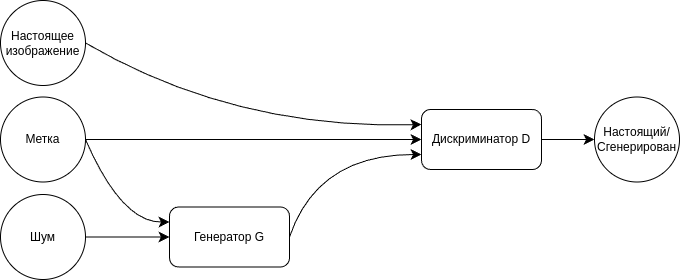
\includegraphics[width=0.75\linewidth]{images/cond_gan.png}
    \caption{Схема условного GAN}
    \label{fig:cond-gan}
\end{figure}

Применяя эту идею, получим следующие целевые функции:
\begin{equation}
    \begin{split}
        B(D, G) = \mathbb{E}_{\pi_T(y)}\mathbb{E}_{p(z)}[D(G(z, y),y)] - \mathbb{E}_{\pi_0(x)}\mathbb{E}_{p(z)}\left[e^{(D(x, K(z, x)) - 1)}\right], \\
        F(T, K) = \mathbb{E}_{\pi_0(x)}\mathbb{E}_{p(z)}[T(x, K(z, x))] - \mathbb{E}_{\pi_T(y)}\mathbb{E}_{p(z)}\left[e^{(T(G(z, y),y) - 1)}\right],
    \end{split}
    \label{eq:objective}
\end{equation}
где $G$ и $K$ -- генераторы, параметризованные нейронными сетями.

Для того, чтобы полноценно реализовать алгоритм IPF с помощью состязательного обучения необходимо проинициализировать $q^0(x|y)$ с помощью условного распределения $p^{\mathbb{W}^\gamma}(y|x) = \mathcal{N}(y| x, \gamma\mathbb{I})$. Для этого на первом шаге обратного прохода будем сэмплировать из заданного априорного распределения, то есть:
\begin{equation*}
    \mathbb{E}_{\pi_T(y)}\mathbb{E}_{p(z)}[D(G(z,y),y)] - \mathbb{E}_{\pi_0(x)}\mathbb{E}_{\mathcal{N}(y| x, \gamma\mathbb{I})}\left[e^{(D(x, y) - 1)}\right].
\end{equation*}
В итоге, получим новый состязательный алгоритм IPF (алгоритм \ref{alg:adv-ipf}).

\begin{algorithm}
\caption{Состязательный IPF}\label{alg:adv-ipf}
\KwInput{$\pi_0(x)$, $\pi_T(y)$, $p(y|x)$}
\KwOutput{$G^i, K^i$}
Инициализируем $i = 0$\;
\While{не сойдется}{
    $G^i = \arg\min_{G}\max_{D}B(D, G)$\;
    $K^i = \arg\min_{K}\max_{T}F(T, K)$\;
    $i:=i+1$\;
   }
\end{algorithm}

Предложенный метод удовлетворяет всем поставленным качествам. Во-первых, отображение происходит за один шаг, так как для того, чтобы отобразить данные из одного распределения в другое, необходимо использовать один раз $G$ или $K$. Во-вторых, в силу того, что метод наследует подход состязательного обучения, результирующая модель хорошо справляется с данными большой размерностью.

\newpage
 %% Описание практической части
    \section{Реализация метода}
\label{sec:Chapter5} \index{Chapter5}

% Перед тем как сформулировать постановку экспериментов и продемонстрировать результаты, аргументируется выбор Python в качестве языка программирования, а PyTorch в качестве фреймворка машинного обучения, для проведения экспериментов.

% \subsection{Выбор языка программирования}
% Выбор Python в качестве языка программирования для глубокого обучения
% Глубокое обучение стало одной из ключевых областей в искусственном интеллекте, и выбор языка программирования играет решающую роль в успехе проектов. Рассмотрим основные языки программирования, используемые в этой области, и обоснуем, почему Python является наиболее предпочтительным.

% \subsubsection{Python}
% Python является наиболее популярным языком для глубокого обучения благодаря своей простоте и широкому спектру библиотек, таких как TensorFlow, Keras и PyTorch. Простота синтаксиса Python позволяет сосредоточиться на алгоритмах и моделях, а не на технических деталях программирования. Кроме того, Python поддерживает объектно-ориентированное, процедурное и функциональное программирование, что делает его универсальным инструментом для различных задач глубокого обучения.

% \subsubsection{C++}
% C++ славится своей скоростью и эффективностью, что делает его хорошим выбором для систем, требующих высокой производительности, таких как роботы и автономные транспортные средства. Однако сложность синтаксиса и время, необходимое на разработку и отладку программ, делают C++ менее привлекательным для исследователей и разработчиков, сосредоточенных на быстром прототипировании и экспериментировании.

% \subsubsection{R}
% R был разработан специально для статистического анализа и визуализации данных, что делает его полезным инструментом для анализа данных и статистического моделирования. Однако для глубокого обучения R уступает Python в плане производительности и наличия специализированных библиотек. Кроме того, синтаксис R считается более сложным для изучения, чем у Python.

% \subsubsection{MATLAB}
% MATLAB предоставляет мощные инструменты для работы с матрицами и числовыми вычислениями, что важно для некоторых аспектов глубокого обучения. Однако его использование ограничено высокими затратами на лицензии и меньшим сообществом пользователей. В то время как MATLAB обладает высокопроизводительными встроенными функциями, Python с его бесплатными библиотеками часто оказывается более экономически эффективным и гибким решением.

% \subsubsection{Java}
% Java известен своей масштабируемостью и надежностью, что делает его подходящим для построения крупномасштабной инфраструктуры ИИ. Однако более сложный синтаксис и необходимость в большем объеме кода по сравнению с Python затрудняют быстрое прототипирование моделей глубокого обучения. Кроме того, экосистема библиотек для глубокого обучения в Java не столь развита, как у Python.

% \subsubsection{Сравнение и выбор}
% Несмотря на преимущества каждого из рассмотренных языков программирования, Python выделяется своей простотой, универсальностью и богатой экосистемой библиотек для глубокого обучения. Эти факторы делают его наиболее подходящим выбором как для начинающих, так и для опытных разработчиков в области глубокого обучения. Python позволяет эффективно разрабатывать, тестировать и внедрять модели глубокого обучения, что подтверждается его широким использованием в академической среде и промышленности.

% \subsection{Выбор фреймворка глубокого обучения}

% Для проведения научного исследования в глубоком обучении требуется мощные и гибкие инструменты для построения и обучения нейронных сетей. Помимо этого, такой фреймворк должен обеспечивать простоту реализации задач для того, чтобы процесс проведения экспериментов не занимал долгое время. Для решения этого вопроса рассмотрим наиболее популярные библиотеки.

% \subsubsection{TensorFlow}
% TensorFlow, разработанный Google, является одним из наиболее популярных фреймворков для глубокого обучения. Он поддерживает как символическое, так и императивное программирование, что позволяет пользователям выбирать между статическим и динамическим построением графов вычислений. TensorFlow широко используется в промышленности благодаря его высокой производительности и возможности развертывания на различных платформах, включая мобильные устройства и серверы.

% Основные преимущества TensorFlow:
% \begin{itemize}
%     \item поддержка распределенных вычислений;
%     \item интеграция с другими инструментами Google, такими как TensorBoard для визуализации и анализа проведенных экспериментов;
%     \item широкая библиотека предварительно обученных моделей.
% \end{itemize}

% Однако, TensorFlow обладает значительной сложностью, особенно для начинающих исследователей, и требует большего объема кода для простых операций.

% \subsubsection{Keras}
% Keras, первоначально разработанный как высокоуровневая библиотека поверх Theano и TensorFlow, стремится упростить разработку моделей глубокого обучения. Он предоставляет удобный и интуитивно понятный интерфейс для создания нейронных сетей.

% Основные преимущества Keras:
% \begin{itemize}
%     \item простота использования и быстрота прототипирования, что полезно для проведения научных исследований;
%     \item поддержка нескольких бэкендов, включая TensorFlow и Theano.
% \end{itemize}

% Тем не менее, ограниченные возможности по сравнению с низкоуровневыми фреймворками могут быть недостатком для сложных и специфических задач.

% \subsubsection{PyTorch}
% PyTorch, разработанный Facebook AI Research, представляет собой фреймворк для глубокого обучения, который стал популярным благодаря своей простоте и гибкости. PyTorch поддерживает динамическое построение графов вычислений, что делает его идеальным для научных исследований и экспериментов.

% Основные преимущества PyTorch:
% \begin{itemize}
%     \item интуитивно понятный и лаконичный синтаксис, напоминающий стандартный Python-код;
%     \item поддержка динамических вычислений, что упрощает отладку и экспериментирование с моделями;
%     \item широкая поддержка сообществом и наличие множества ресурсов для обучения и примеров.
% \end{itemize}

% \subsubsection{JAX}
% JAX, разработанный Google Research, представляет собой мощный инструмент для численных вычислений и машинного обучения, который сочетает в себе возможности библиотек Autograd и XLA. В данном обзоре рассмотрим особенности и преимущества JAX, а также его применение и отличия от PyTorch.

% JAX предлагает API, схожий с NumPy, но с возможностью выполнения вычислений на GPU и TPU, что значительно ускоряет процессы. Основные функции JAX включают:

% Преимущества JAX:
% \begin{itemize}
%     \item \textbf{производительность}: Благодаря компилятору XLA, JAX обеспечивает высокую производительность и оптимизацию вычислений на GPU и TPU;
%     \item гибкость: Позволяет исследователям легко экспериментировать с новыми архитекторами моделей и алгоритмами.
% \end{itemize}

% \subsubsection{Сравнение и выбор}
% Для научных экспериментов в области глубокого обучения ключевыми факторами являются простота использования, гибкость, поддержка сообществом и возможности для прототипирования. PyTorch выделяется среди других фреймворков благодаря:
% \begin{itemize}
%     \item интуитивно понятному и читаемому коду, что снижает порог вхождения для начинающих исследователей;
%     \item динамическому построению графов вычислений, что упрощает отладку и экспериментирование;
%     \item активному сообществу и большому количеству образовательных ресурсов, что способствует быстрому освоению и применению фреймворка.
% \end{itemize}

% Исходя из рассмотренных факторов, PyTorch является наиболее подходящим инструментом для научных экспериментов в сфере глубокого обучения. Его простота, гибкость и поддержка сообществом делают его идеальным выбором для исследователей, стремящихся к быстрому прототипированию и адаптации моделей. Несмотря на сильные стороны TensorFlow и других фреймворков, PyTorch обеспечивает оптимальный баланс между функциональностью и удобством использования, что критически важно в научной работе.

\subsection{Эксперименты}
Для эмпирического подтверждения факта, что данный метод решения задачи мостов Шрёдингера удовлетворяет поставленным требованиям, рассматриваются два эксперимента:
\begin{itemize}
    \item эксперимент на 2D данных;
    \item эксперимент на EMNIST.
\end{itemize}
Все эксперименты доступны в github репозитории\footnote{https://github.com/gregkseno/masters-thesis/tree/master}.

\subsubsection{2D данные}
Перед проверкой метода на данных большой размерности, проводится эксперимент на 2D данных, который предназначен, во-первых, для санитарного теста работоспособности метода, а, во-вторых, для проверки способности отображения при различных параметрах $\gamma$.

\begin{figure}
    \centering
    \subfloat[Кольца]{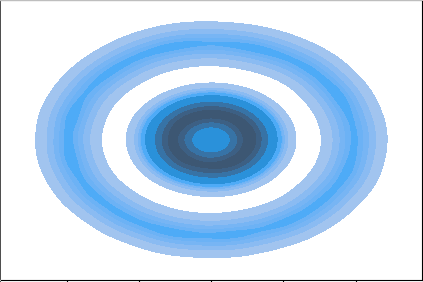
\includegraphics[width=0.4\linewidth]{images/circles.png}}
    \hfill
    \subfloat[Луны]{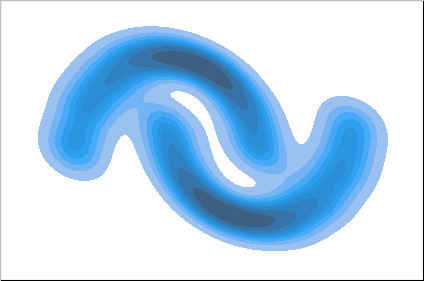
\includegraphics[width=0.4\linewidth]{images/moons.png}}   
    \subfloat[Рулет]{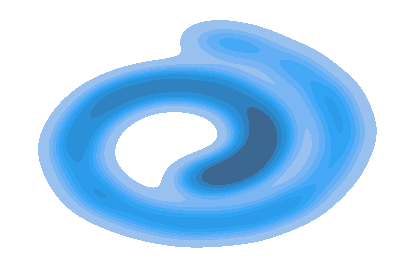
\includegraphics[width=0.4\linewidth]{images/swiss_roll.png}}   
    \caption{Набор 2D данных}
    \label{fig:moons-circles}
\end{figure}

Данными для 2D экспериментов послужили наборы из библиотеки sci-kit learn, а именно кольца, луны и рулет (рисунок \ref{fig:moons-circles}). Данные наборы представляют собой набор пар координат точек в плоскости.

Для санитарной проверки были выбраны кольца и луны в качестве $X$ и $Y$, соответственно. Для формирования набора лун были использованы следующие параметры:
\begin{itemize}
    \item количество точек обучающей выборки: $5000$;
    \item параметр стандартного отклонения шума, добавленного к данным: $0.05$
\end{itemize}

Для колец выбраны следующие параметры:
\begin{itemize}
    \item количество точек обучающей выборки: $5000$;
    \item параметр стандартного отклонения шума, добавленного к данным: $0.03$
    \item расстояние от между кольцами: $0.3$
\end{itemize}

Генератор параметризуется с помощью $3$-х полно-связных слоев. Каждый слой имеет $256$ нейронов. ReLU был выбран в качестве желаемой функции активации.

Для параметризации дискриминатора используется почти та же архитектура: $3$ полно-связных слоя со скрытыми слоем размером $256$, однако вместо ReLU, функцией активации является LeakyReLU с коэффициентом угла $0.2$. На вход подается конкатенация элементов из $X$ и $Y$, а на выходе скаляр. 

Также для лучшей сходимости после каждого линейного слоя генератора и дискриминатора применялась послойная нормализация.

Параметры оптимизаторов были выбраны следующие: 
\begin{itemize}
    \item используется AdamW в качестве алгоритма оптимизации;
    \item коэффициентом L2 регуляризации является значение $0,1$ для генератора и для дискриминатора;
    \item скорости обучения были установлены $1e-6$ для генераторов и дискриминаторов;
    \item размер батча был выбран $1024$
    \item модели обучались на протяжении $400$ эпох, а количество шагов состязательного обучения составило $60$;
    \item в качестве параметра $\gamma$ было выбрано значение $0.1$.
\end{itemize}

\begin{figure}
    \centering
    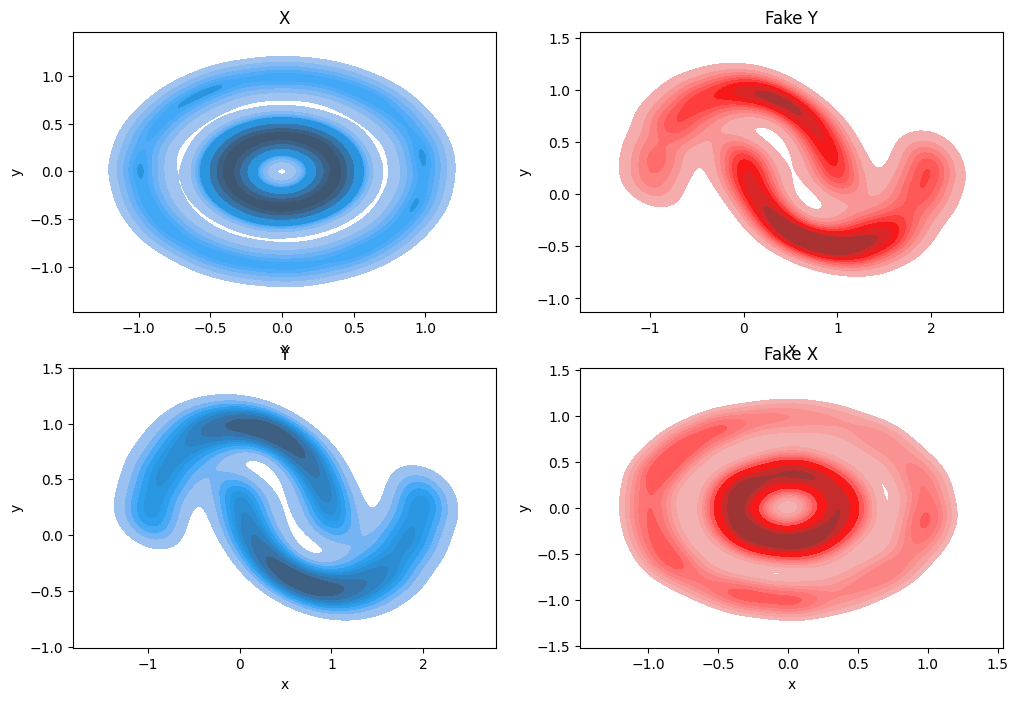
\includegraphics[width=1\linewidth]{images/2d_results.png}
    \caption{Результаты трансляции на кольцах, $X$, и  лунах, $Y$, с $\gamma = 0.1$}
    \label{fig:2d-res}
\end{figure}

Из результатов, изображенных на рисунке \ref{fig:2d-res}, понятно, что метод хорошо справляется с данными распределениями. Помимо визуального сходства, также можно заметить, что метод не сжимает или разжимает маргинальные распределения, таким образом сгенерированные элементы распределены с теми же средним и дисперсией.

Для сравнения трансляций при различных $\gamma$ 2D данных был выбраны стандартная гауссиана и рулет, для $X$ и $Y$, соответственно. Для рулета выбраны следующие параметры:
\begin{itemize}
    \item количество точек обучающей выборки: $5000$;
    \item параметр стандартного отклонения шума, добавленного к данным: $0.5$
\end{itemize}

\begin{figure}
    \centering
    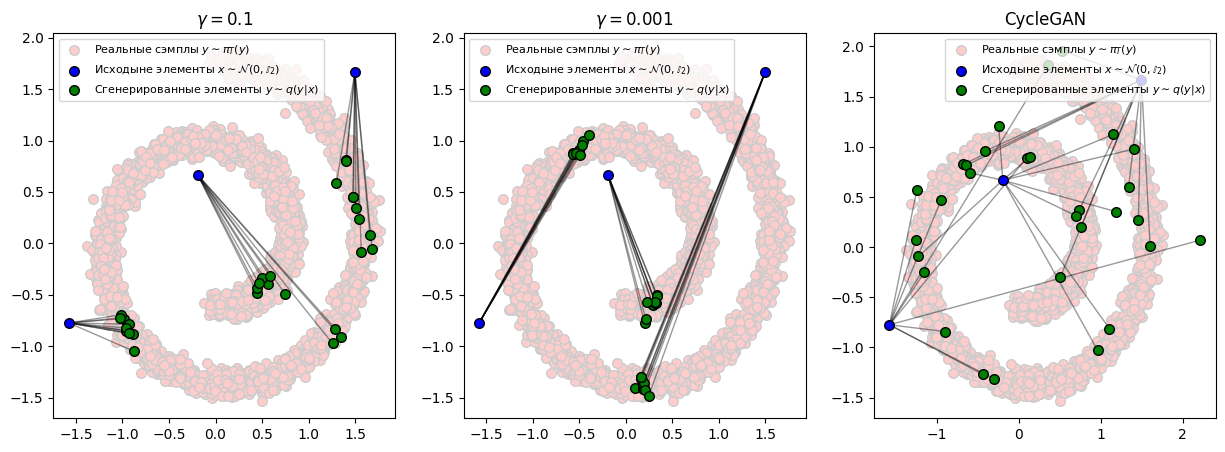
\includegraphics[width=1\linewidth]{images/2d_gamma.png}
    \caption{Сравнение трансляций точек предложенного метода с различными $\gamma$ и CycleGAN}
    \label{fig:2d-gamma}
\end{figure}

Целью данного эксперимента является анализ различия трансляций предложенного метода с различными $\gamma$ и CycleGAN \cite{cycle-gan}. Для этого эксперимента главным гиперпараметром является $\gamma$. В монографии \cite{monography-sbp} показано, что некоторые методы работают при больших $\gamma = 1000$, а некоторые — при низких $\gamma = 1$. Меньшее значение $\gamma$ гарантирует меньшее разброс отображенных элементов, то есть менее разнообразный вывод. В экскрементах были протестированы следующие параметры $\gamma$: $0.1$ и $0.001$.

Результаты (рисунок \ref{fig:2d-gamma}) демонстрируют, что метод отлично справляется с малыми параметрами $\gamma$. Также можно заметить, что при различных $\gamma$, действительно, отображение становится менее разнообразным. Более того, сравнивая предложенный метод с CycleGAN, транслированные элементы находятся в некоторой окрестности друг от друга, что не скажешь про трансляции CycleGAN.

\subsubsection{EMNIST}

\begin{figure}
    \centering
    \subfloat[Трансляция из букв в цифры]{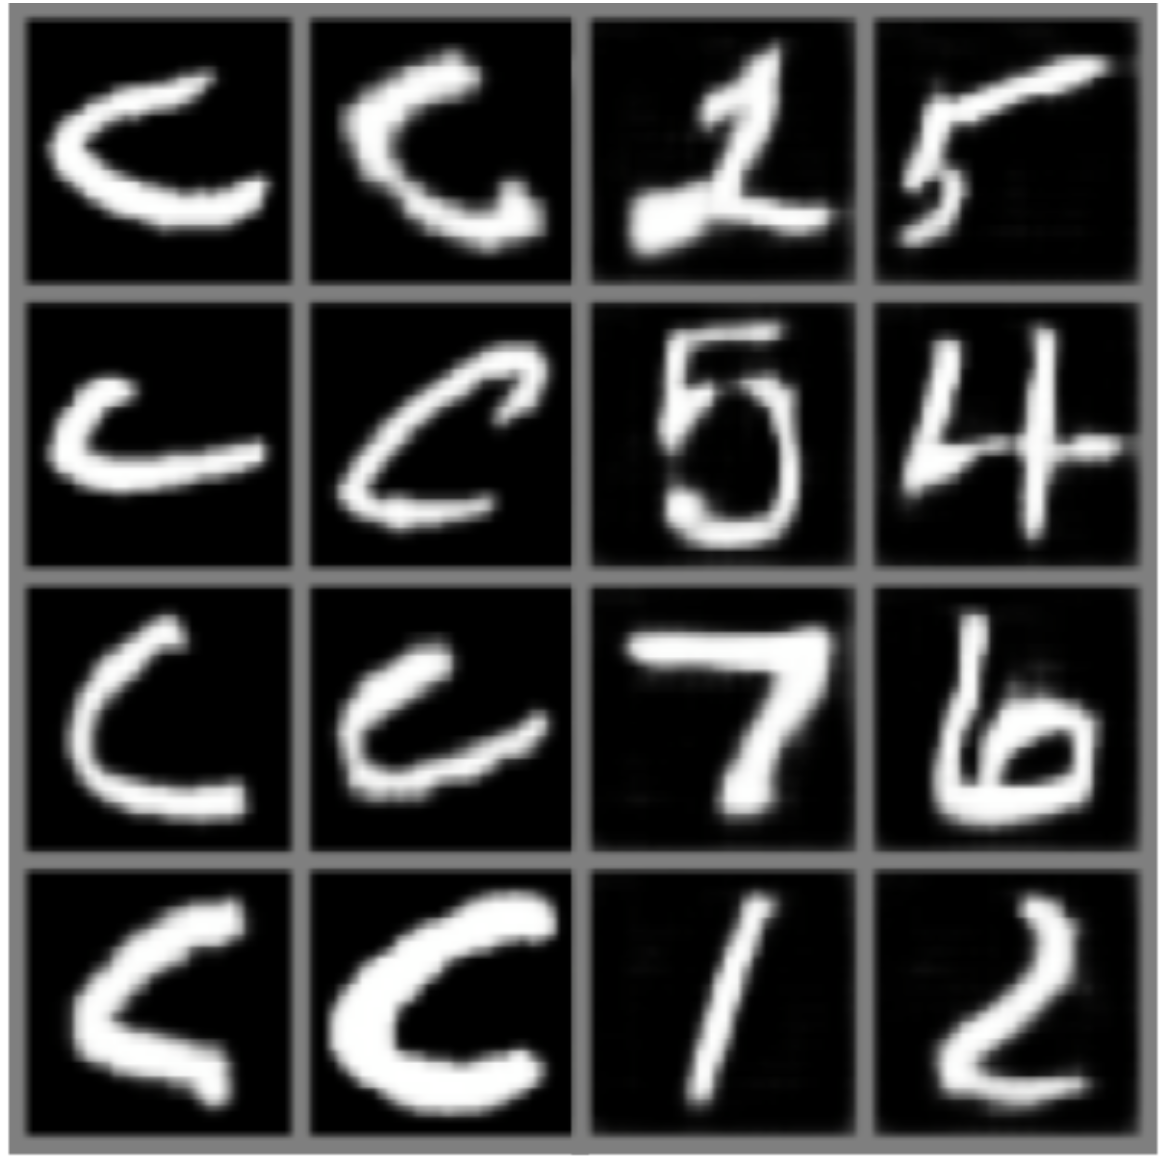
\includegraphics[width=0.4\linewidth]{images/emnist_cond_p.png}}
    \hfill
    \subfloat[Трансляция из цифр в буквы]{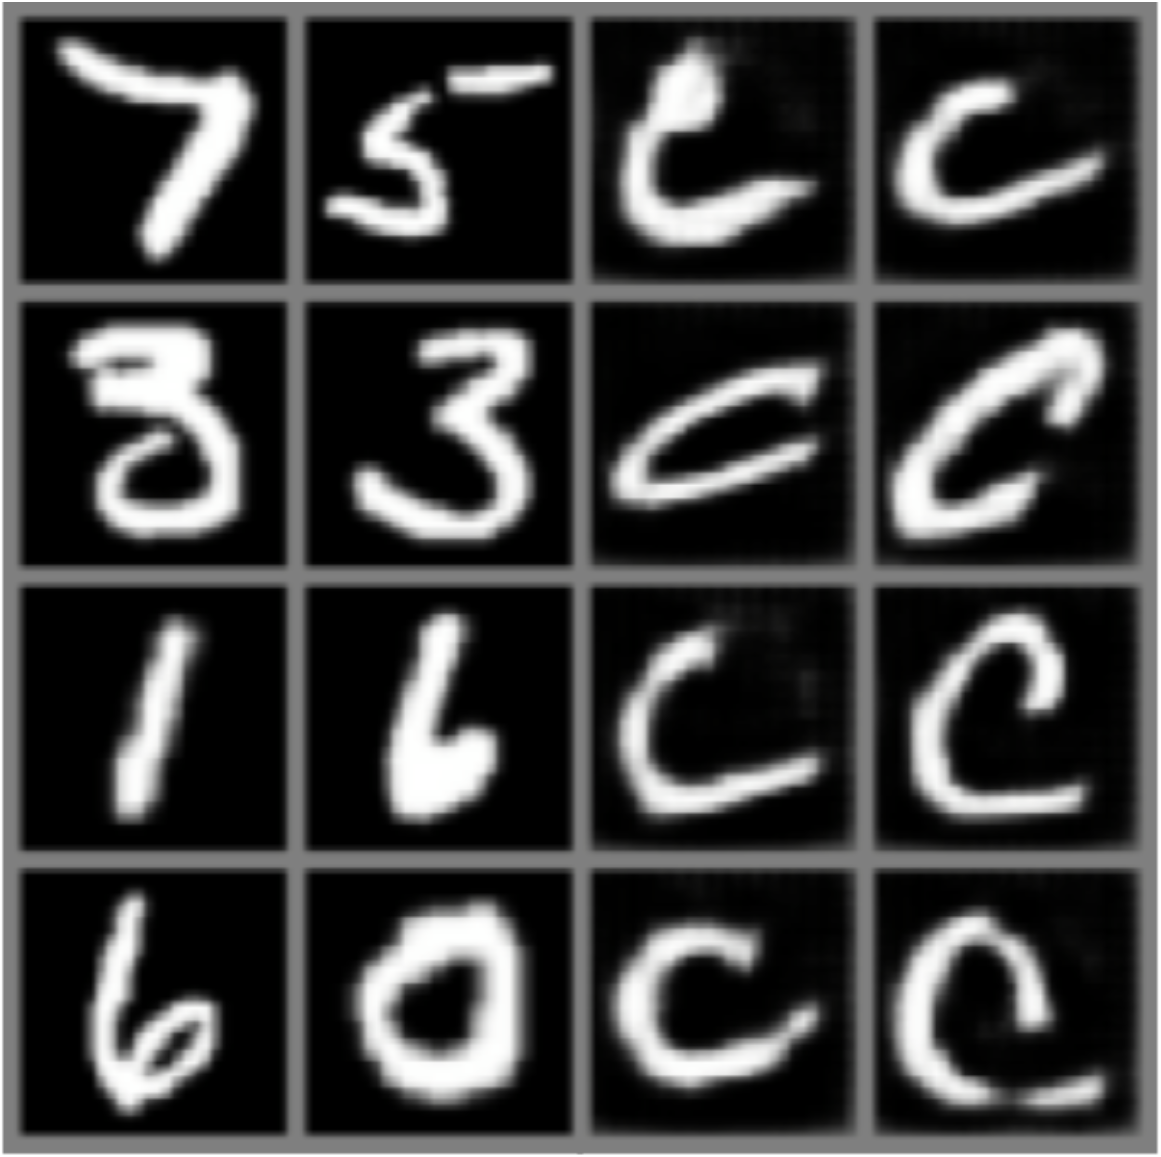
\includegraphics[width=0.4\linewidth]{images/emnist_cond_q.png}}  
    \caption{Пример трансляции на набор данных EMNIST}
    \label{fig:emnist-res}
\end{figure}

Целью данного эксперимента является подтверждение того факта, что метод работает на данных большой размерностью. Для этого был выбран набор данных EMNIST, который представляет собой набор рукописных символов, полученных из специальной базы данных NIST 19 и преобразованных в формат изображения 28x28 пикселей и структуру набора данных, которая напрямую соответствует набору данных MNIST.

В качестве набора $X$ был выбран поднабор EMNIST, а именно 145,600 латинских рукописных букв с 26 классами. В качестве $Y$ был выбран классический MNIST, в котором 70,000 цифр. Классы обоих наборов были сбалансированы. 

В качестве архитектуры генератора и дискриминатора для данного эксперимента использовались сверхточные слои с нормализацией по батчу, с вероятностью дропаута $0.2$, а также с функцией активации LeakyReLU с углом наклона $0.2$. Чтобы соответствовать области определения изображений $[0, 1]$, последней функцией генератора была выбрана гиперболический тангенс. Полную архитектуру можно посмотреть на рисунках \ref{fig:gen}, \ref{fig:disc}.

\begin{figure}
    \centering
    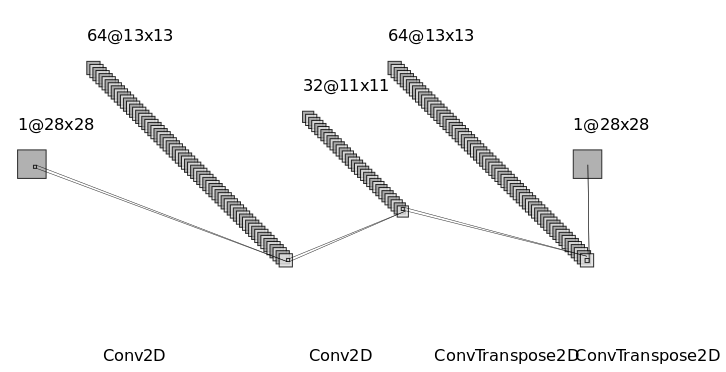
\includegraphics[width=0.8\linewidth]{images/generator.png}
    \caption{Архитектура генератора}
    \label{fig:gen}
\end{figure}

\begin{figure}
    \centering
    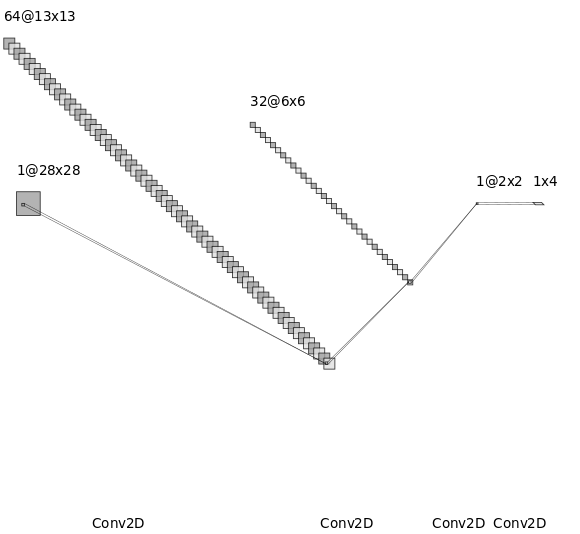
\includegraphics[width=0.6\linewidth]{images/disc.png}
    \caption{Архитектура дискриминатора}
    \label{fig:disc}
\end{figure}

Параметры оптимизаторов были выбраны следующие: 
\begin{itemize}
    \item используется AdamW в качестве алгоритма оптимизации;
    \item коэффициентом L2 регуляризации является значение $0,1$ для генератора и для дискриминатора;
    \item скорости обучения были установлены $1e-5$ для генераторов и дискриминаторов;
    \item размер батча был выбран $4096$
    \item модели обучались на протяжении $300$ эпох, а количество шагов состязательного обучения составило $60$;
    \item в качестве параметра $\gamma$ было выбрано значение $1$.
\end{itemize}

Результаты данного эксперимента продемонстрированы на рисунке \ref{fig:emnist-res}. Таким образом, можно заключить, что данный метод справляется с данными большой размерностью.

Также стоит отметить, что размерность 28x28 не является действительно большой и предыдущие методы, например Diffusion Schrödinger Bridge, также в качестве данных для экспериментов использовали EMNIST. Ожидается, что предложенный метод также можно использовать на данных большей размерностью, однако проведение таких экспериментов было не возможно в силу отсутствия вычислительных ресурсов.

\newpage
 %% Заключение
    \section{Заключение}
\label{sec:Chapter6} \index{Chapter6}

В ходе выполнения данной магистерской диссертации были достигнуты следующие результаты:
\begin{enumerate}
    \item Проведен обзор и анализ различных подходов к решению задачи мостов Шрёдингера, включая Data Driven Schrödinger Bridge, Light Schrödinger Bridge, Diffusion Schrödinger Bridge, Iterative Proportional Maximum Likelihood (IPML) и Unpaired Neural Schrödinger Bridge.
    \item Предложен метод состязательных мостов Шрёдингера, объединяющий идеи генеративных состязательных сетей (GAN) и задачу мостов Шрёдингера.
    \item Проведен эксперимент на 2D данных с использованием наборов данных кольца, луны и рулета из библиотеки sci-kit learn. Параметры набора данных были выбраны таким образом, чтобы проверить работоспособность метода и его способность к отображению при различных параметрах $\gamma$, а также проверить оптимальность отображения, что подтверждает пригодность предложенного метода для решения задачи мостов Шрёдингера.
    \item Проведено сравнение отображений CycleGAN и предложенного метода.
    \item Проведен эксперимент на данных большой размерности с использованием набора данных EMNIST, который подтверждает способность метода работать с большими и сложными наборами данных.
\end{enumerate}

В итоге, можно заключить, что задача, поставленная в данной магистерской диссертации, была решена в полной мере. Разработанный метод состязательных мостов Шрёдингера доказал свою эффективность и применимость для задач трансляции доменов. Проведенные эксперименты подтвердили теоретические выводы и продемонстрировали высокую эффективность предложенного подхода. В будущем данный метод может быть расширен и адаптирован для решения более широкого круга задач в области машинного обучения и анализа данных.

\newpage
 %% Заключение

    %% НЕ ТРОГАЙТЕ!!!
    \nocite{*}
    \bibliography{references}

    %% в зависимости от надобности подключаем раздел "Приложение"
    % \newpage
    % \section*{Приложение}
\addcontentsline{toc}{section}{Приложение}
\label{sec:Apendix} \index{Apendix}

Здесь необходимо написать приложение, которое вы должны придумать самостоятельно.

\end{document}
